\cleardoublepage
\chapter{HASIL IMPLEMENTASI}

Lampiran ini menyajikan tangkapan layar (\textit{screenshot}) hasil implementasi antarmuka \textit{front-end} aplikasi \textit{tracker} ITB Ultra-Marathon pada dua platform, yaitu aplikasi \textit{mobile} dan aplikasi web.

% ============================================================
\section*{A.1 Aplikasi \textit{Mobile}}
\addcontentsline{toc}{section}{A.1 Aplikasi \textit{Mobile}}
% ============================================================

\begin{longtable}{|>{\raggedright\arraybackslash}p{3.8cm}|c|}
\caption*{Tabel A.1 Hasil Implementasi Antarmuka Aplikasi \textit{Mobile}} \\
\hline
\textbf{Fitur} & \textbf{Gambar} \\ \hline
\endfirsthead
\hline
\textbf{Fitur} & \textbf{Gambar} \\ \hline
\endhead
\hline
\endfoot
\hline
\endlastfoot

Halaman Utama Pelari saat GPS aktif dan pelari sedang berlari (\textit{Active State}) &
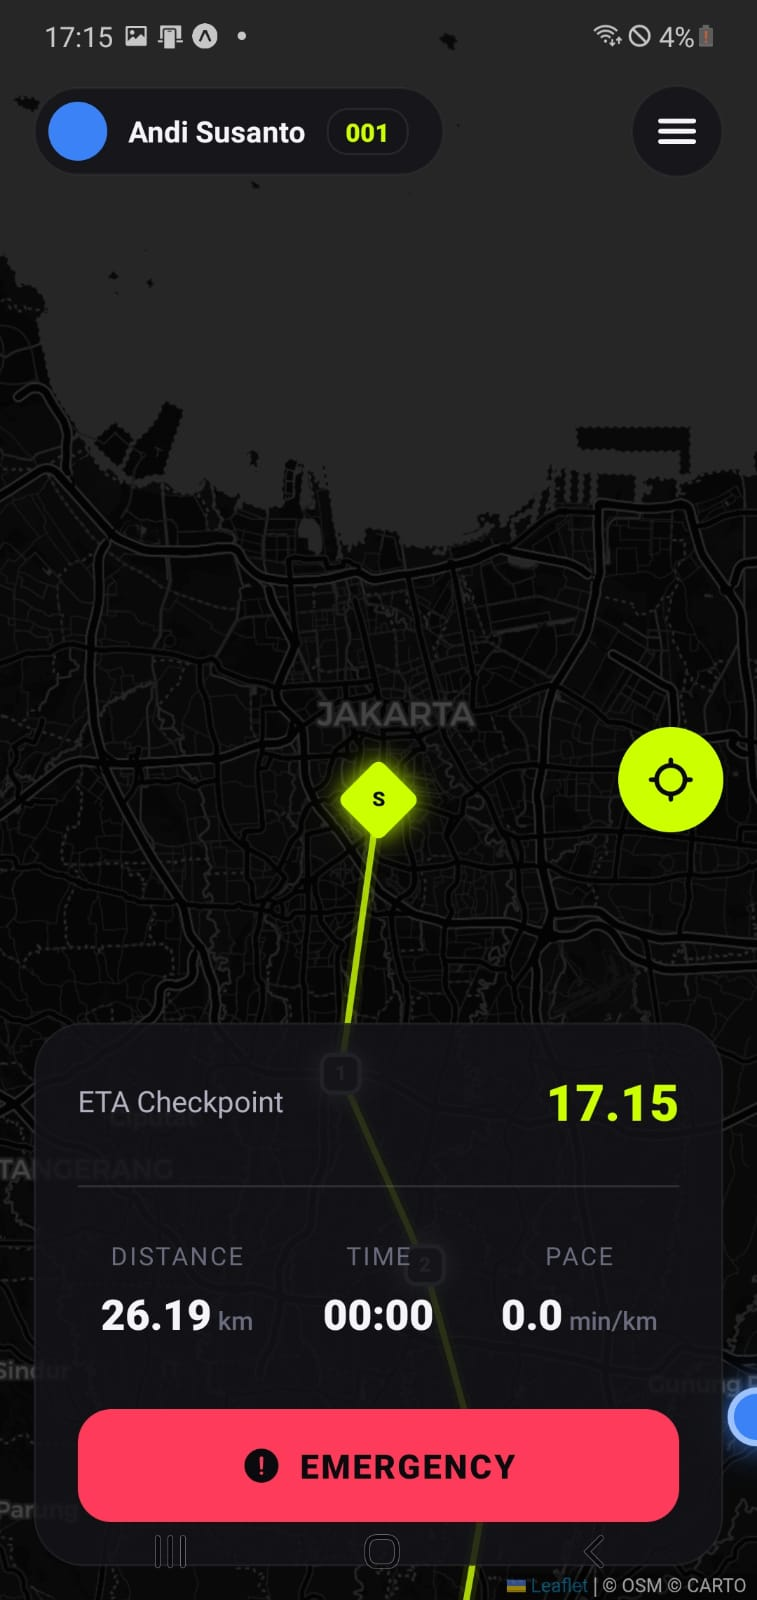
\includegraphics[height=8cm,keepaspectratio]{images/implementasi/mobile/Active.jpeg} \\ \hline

Halaman Utama Pelari saat GPS belum aktif atau pelari sedang menunggu giliran (\textit{Inactive State}) &
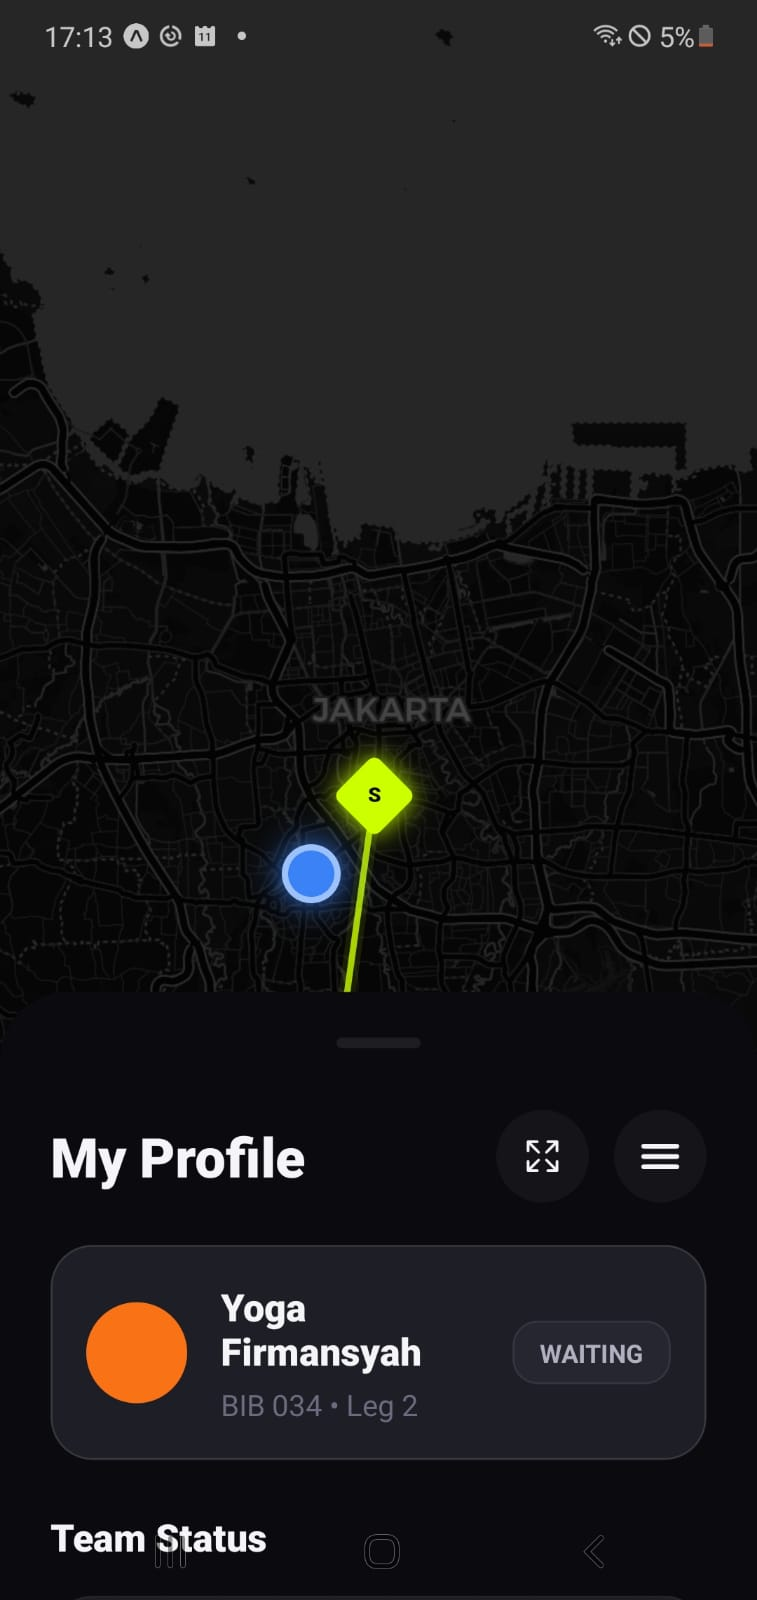
\includegraphics[height=8cm,keepaspectratio]{images/implementasi/mobile/Inactive.jpeg} \\ \hline

Halaman Darurat yang menampilkan tombol SOS dan tombol LOST untuk mengirim sinyal darurat ke panitia &
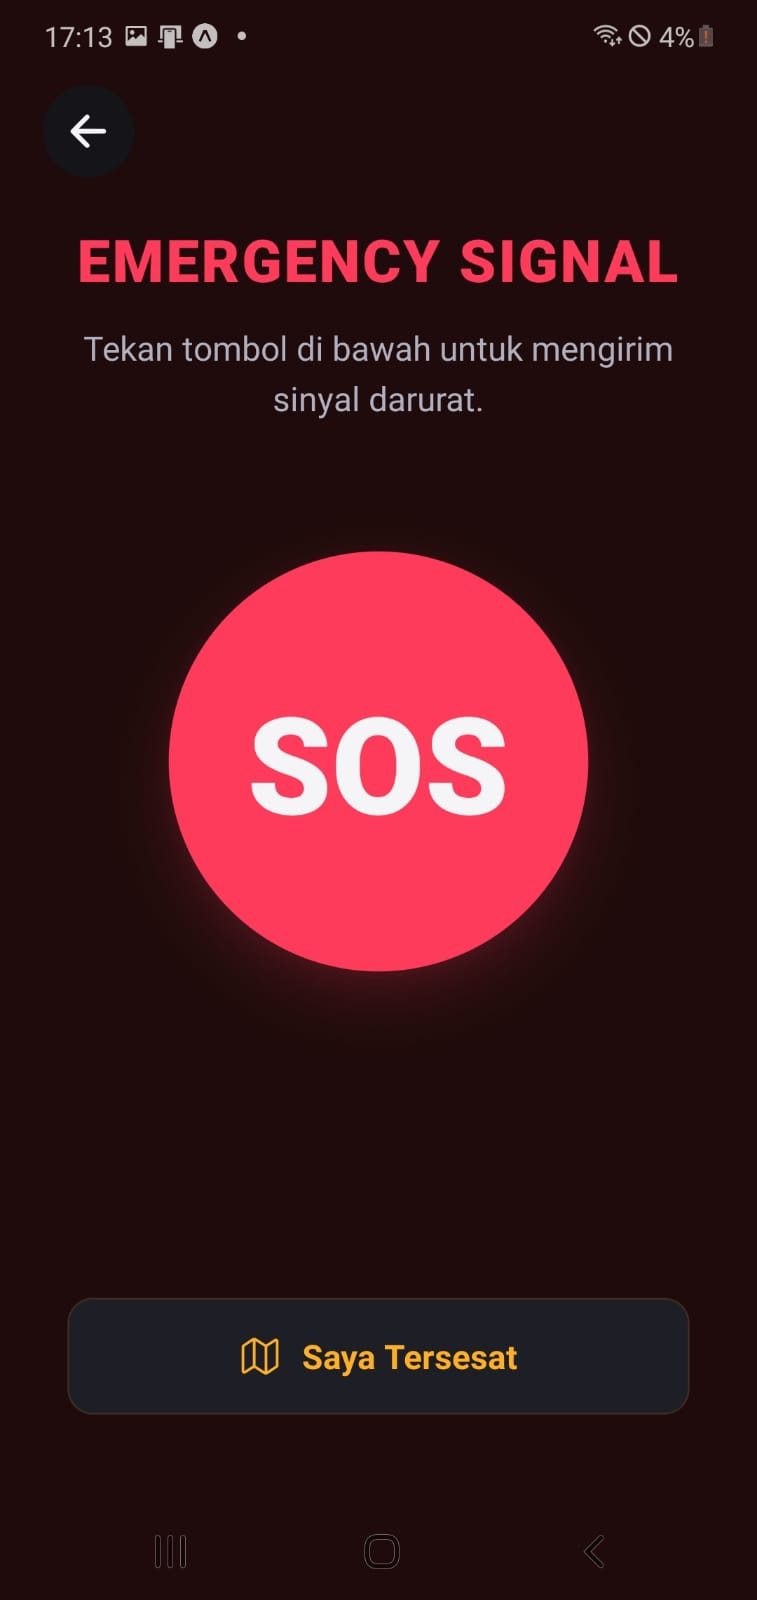
\includegraphics[height=8cm,keepaspectratio]{images/implementasi/mobile/Emergency.jpeg} \\ \hline

Halaman Menu yang menyediakan pengaturan visibilitas (\textit{public/private}) dan fitur pendukung lainnya &
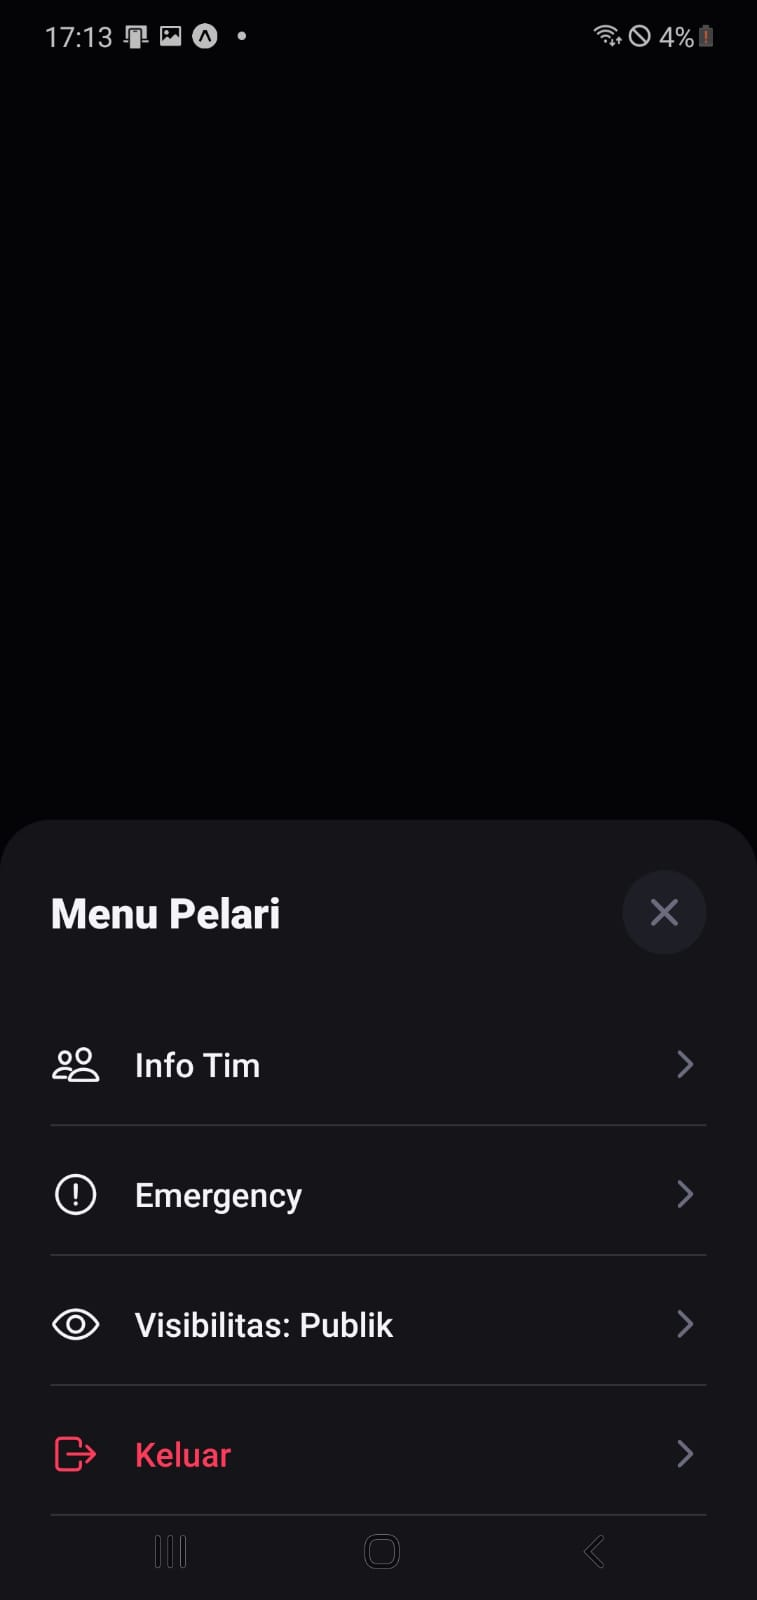
\includegraphics[height=8cm,keepaspectratio]{images/implementasi/mobile/Menu.jpeg} \\ \hline

Halaman Info Tim yang menampilkan status dan posisi anggota tim \textit{relay} secara \textit{real-time} &
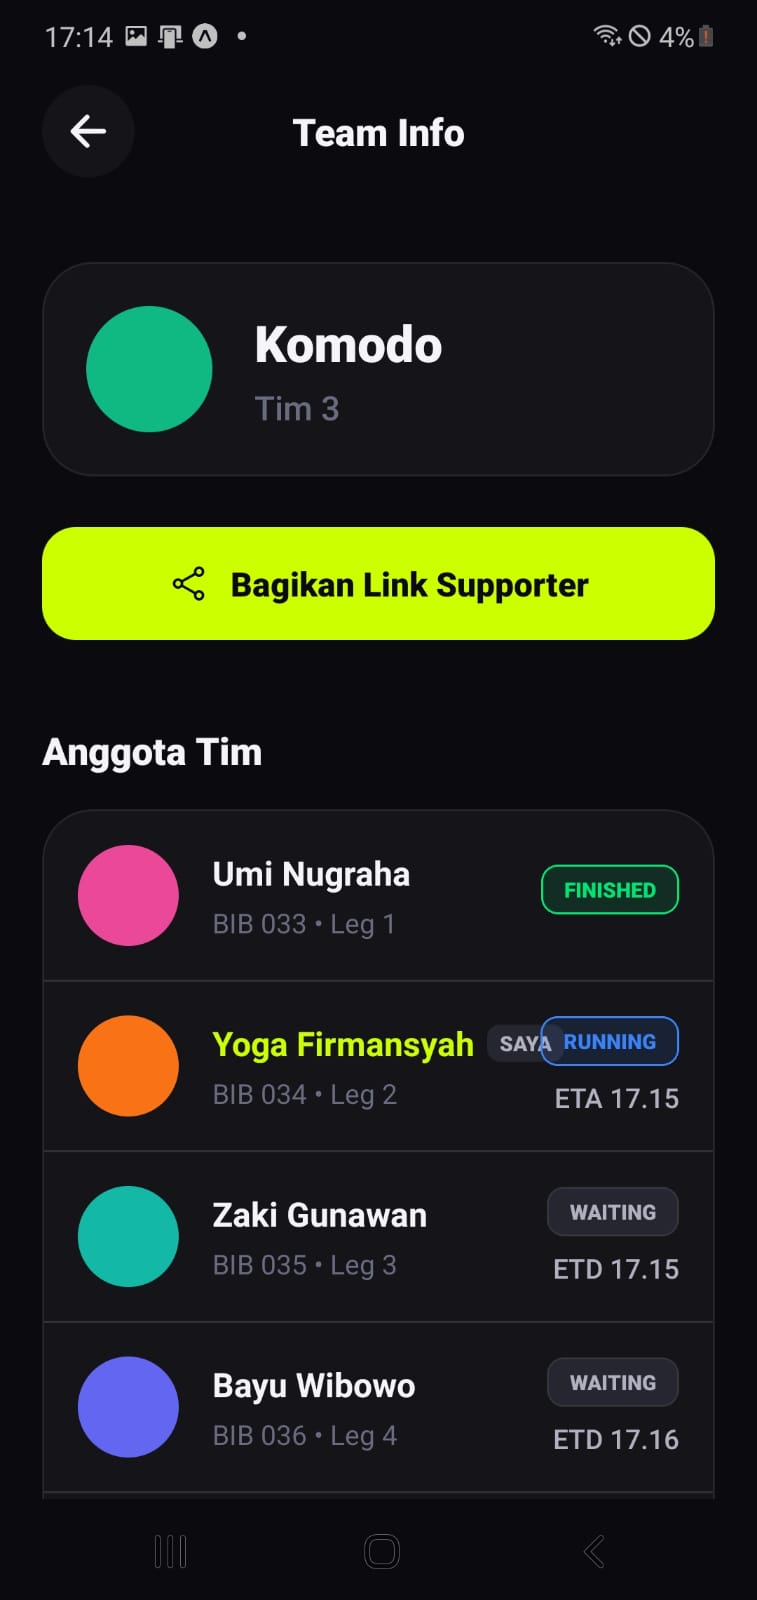
\includegraphics[height=8cm,keepaspectratio]{images/implementasi/mobile/TeamInfo.jpeg} \\

\end{longtable}

% ============================================================
\section*{A.2 Aplikasi Web --- Halaman Publik}
\addcontentsline{toc}{section}{A.2 Aplikasi Web --- Halaman Publik}
% ============================================================

\begin{longtable}{|>{\raggedright\arraybackslash}p{3.8cm}|c|}
\caption*{Tabel A.2 Hasil Implementasi Antarmuka Web --- Halaman Publik} \\
\hline
\textbf{Fitur} & \textbf{Gambar} \\ \hline
\endfirsthead
\hline
\textbf{Fitur} & \textbf{Gambar} \\ \hline
\endhead
\hline
\endfoot
\hline
\endlastfoot

Halaman utama \textit{Public Tracking} yang menampilkan peta interaktif beserta posisi seluruh pelari yang mengaktifkan visibilitas publik &
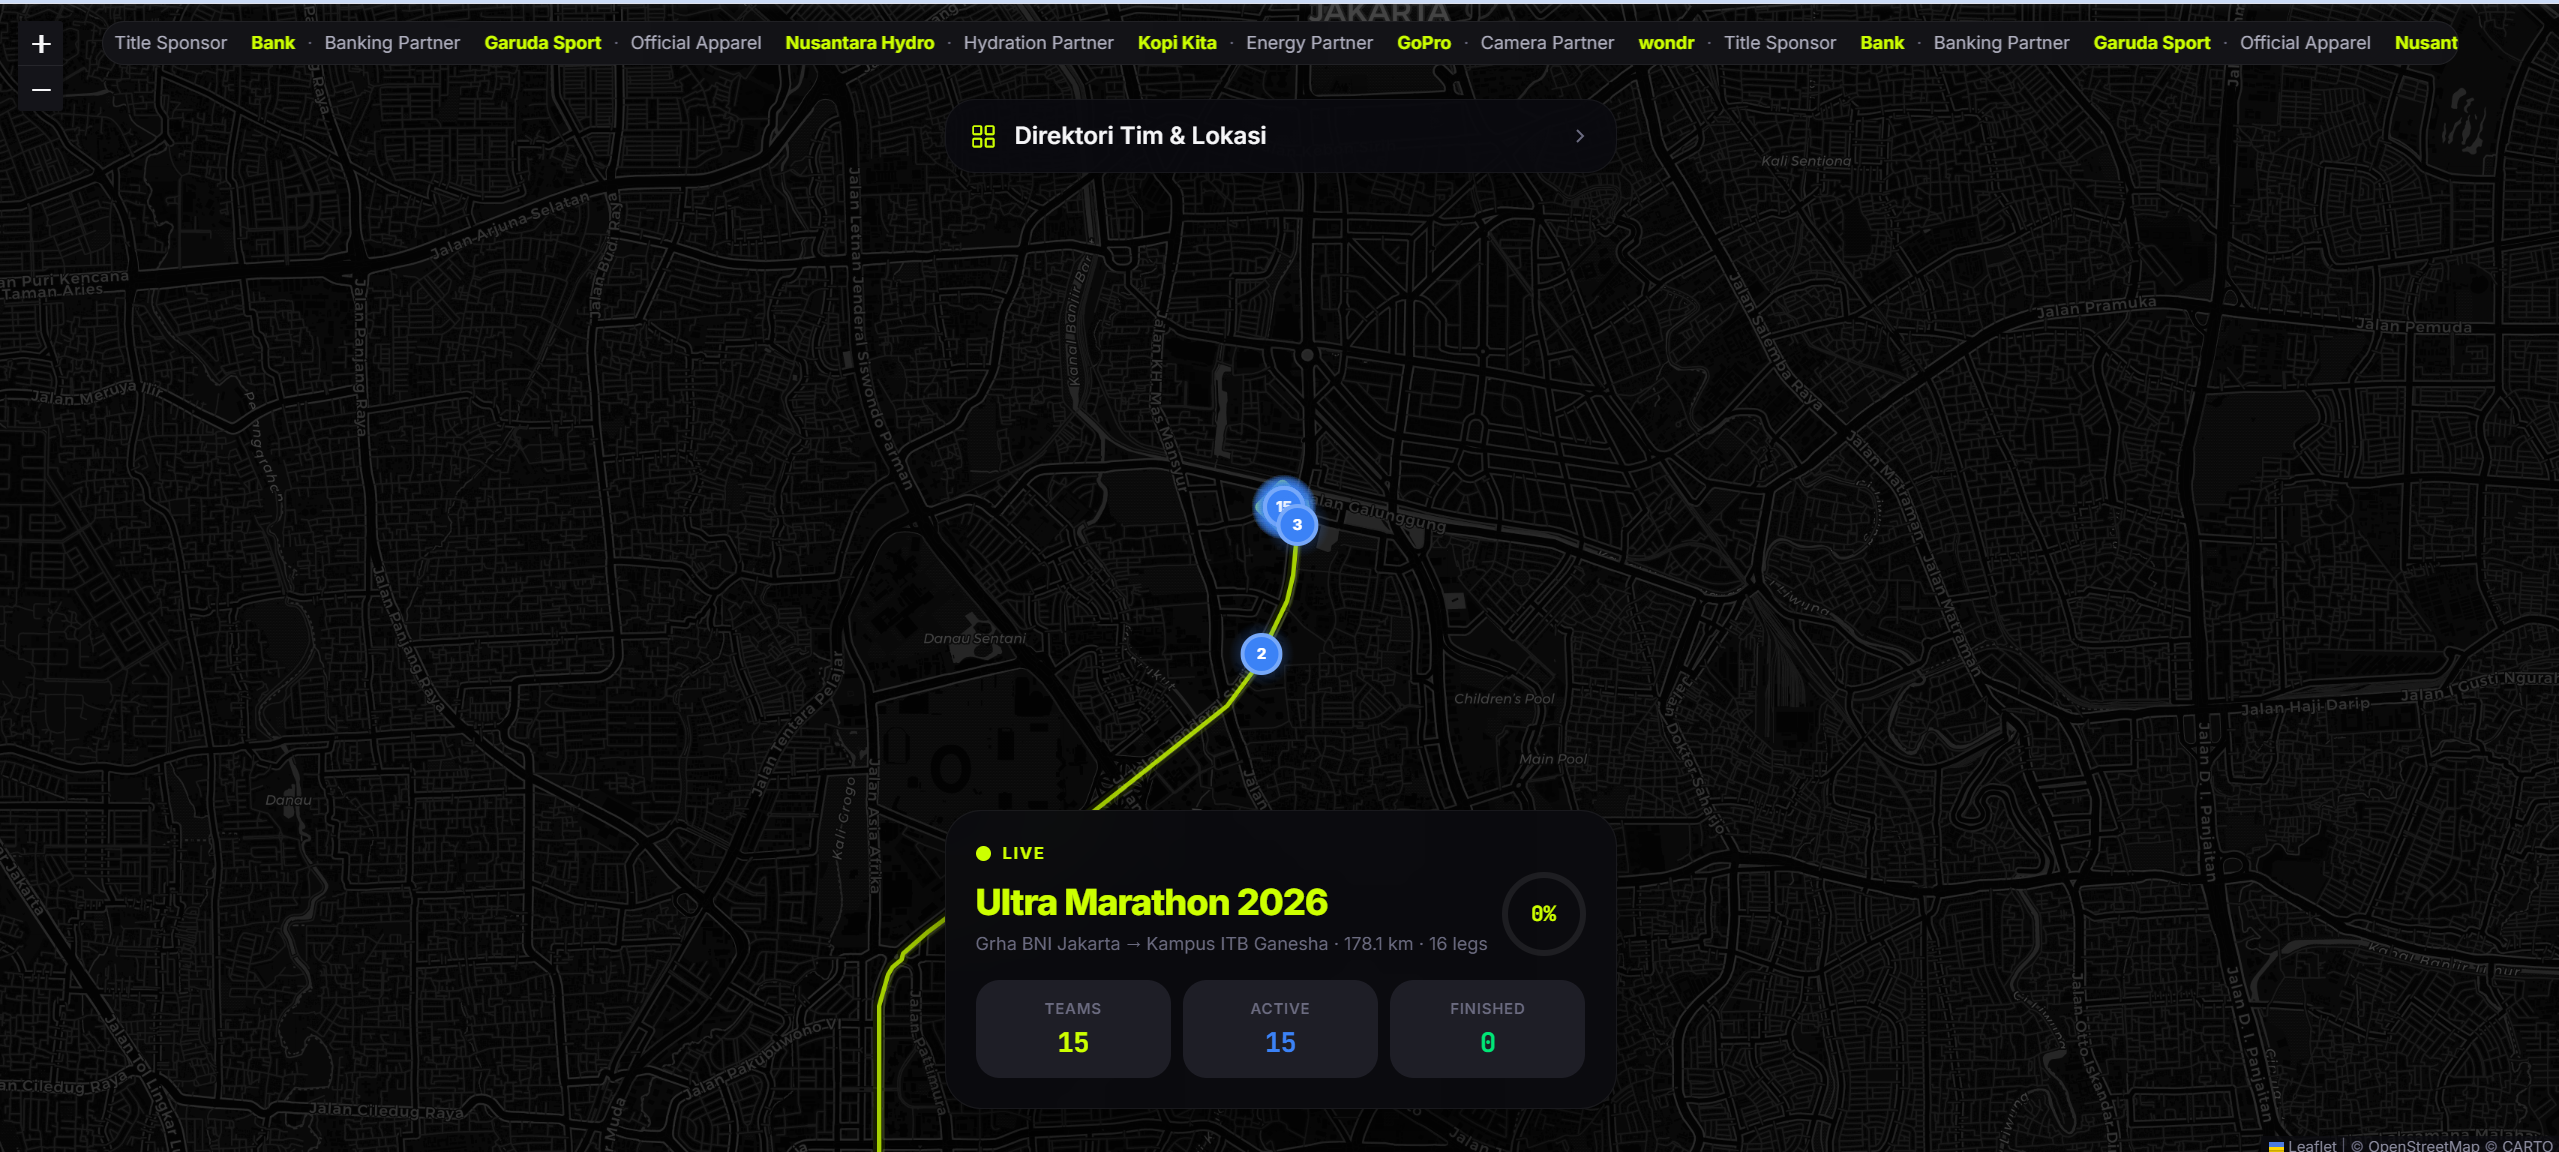
\includegraphics[width=0.62\textwidth,keepaspectratio]{images/implementasi/web/public-home.png} \\ \hline

Panel detail pelari yang muncul saat pengguna mengeklik penanda (\textit{marker}) pelari pada peta &
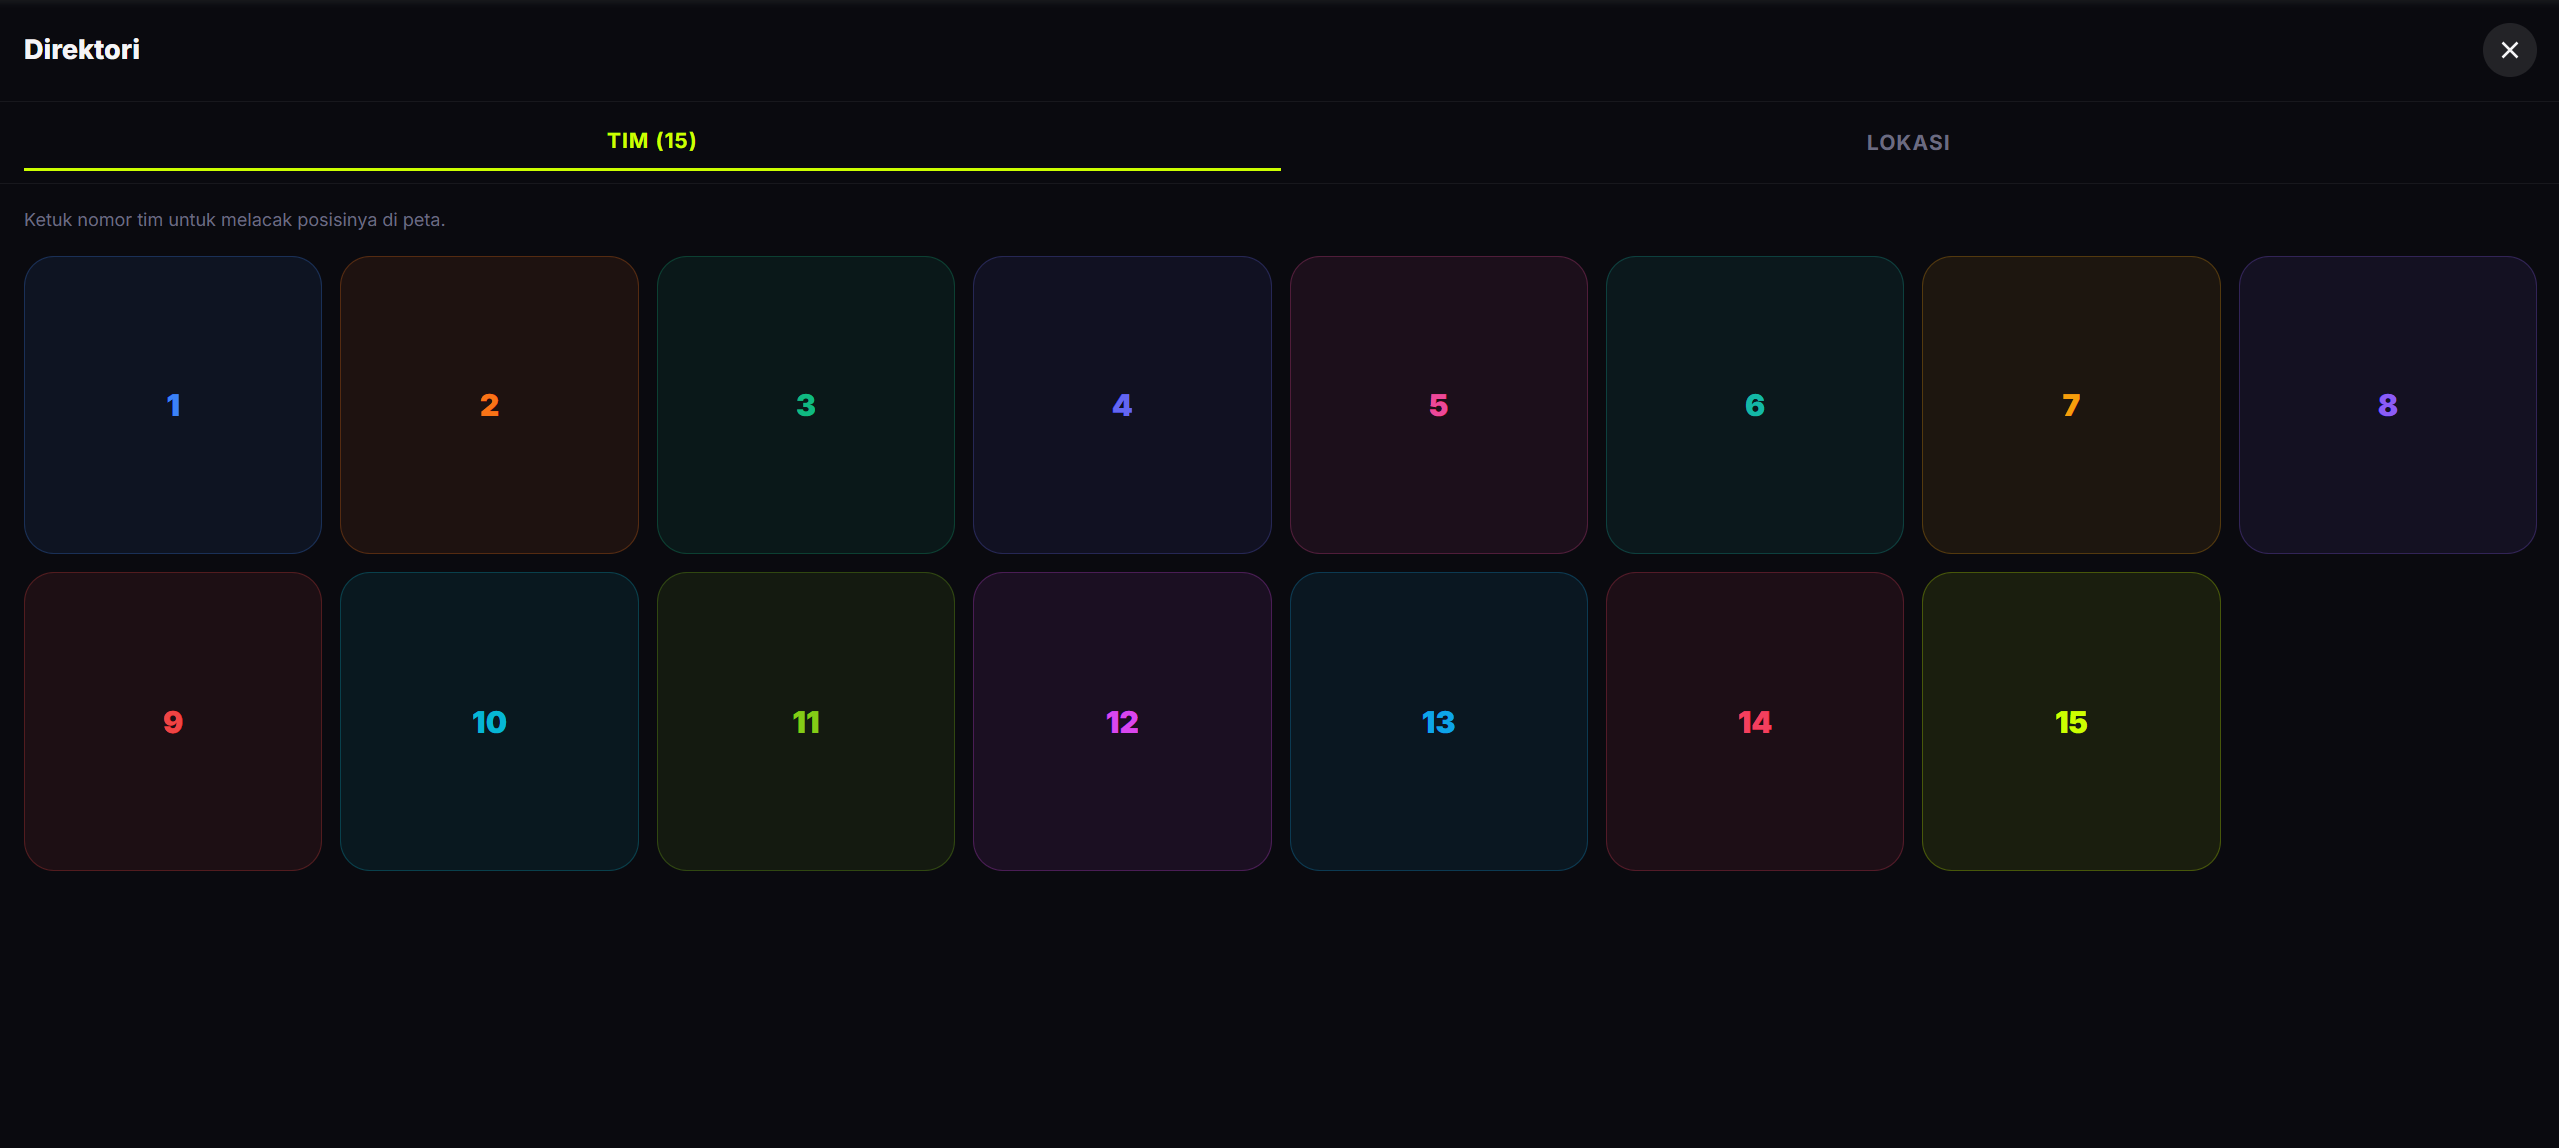
\includegraphics[width=0.62\textwidth,keepaspectratio]{images/implementasi/web/public-runner.png} \\ \hline

Fitur direktori lokasi yang memungkinkan pengguna mencari dan mengarahkan peta ke titik \textit{water station} atau tim tertentu &
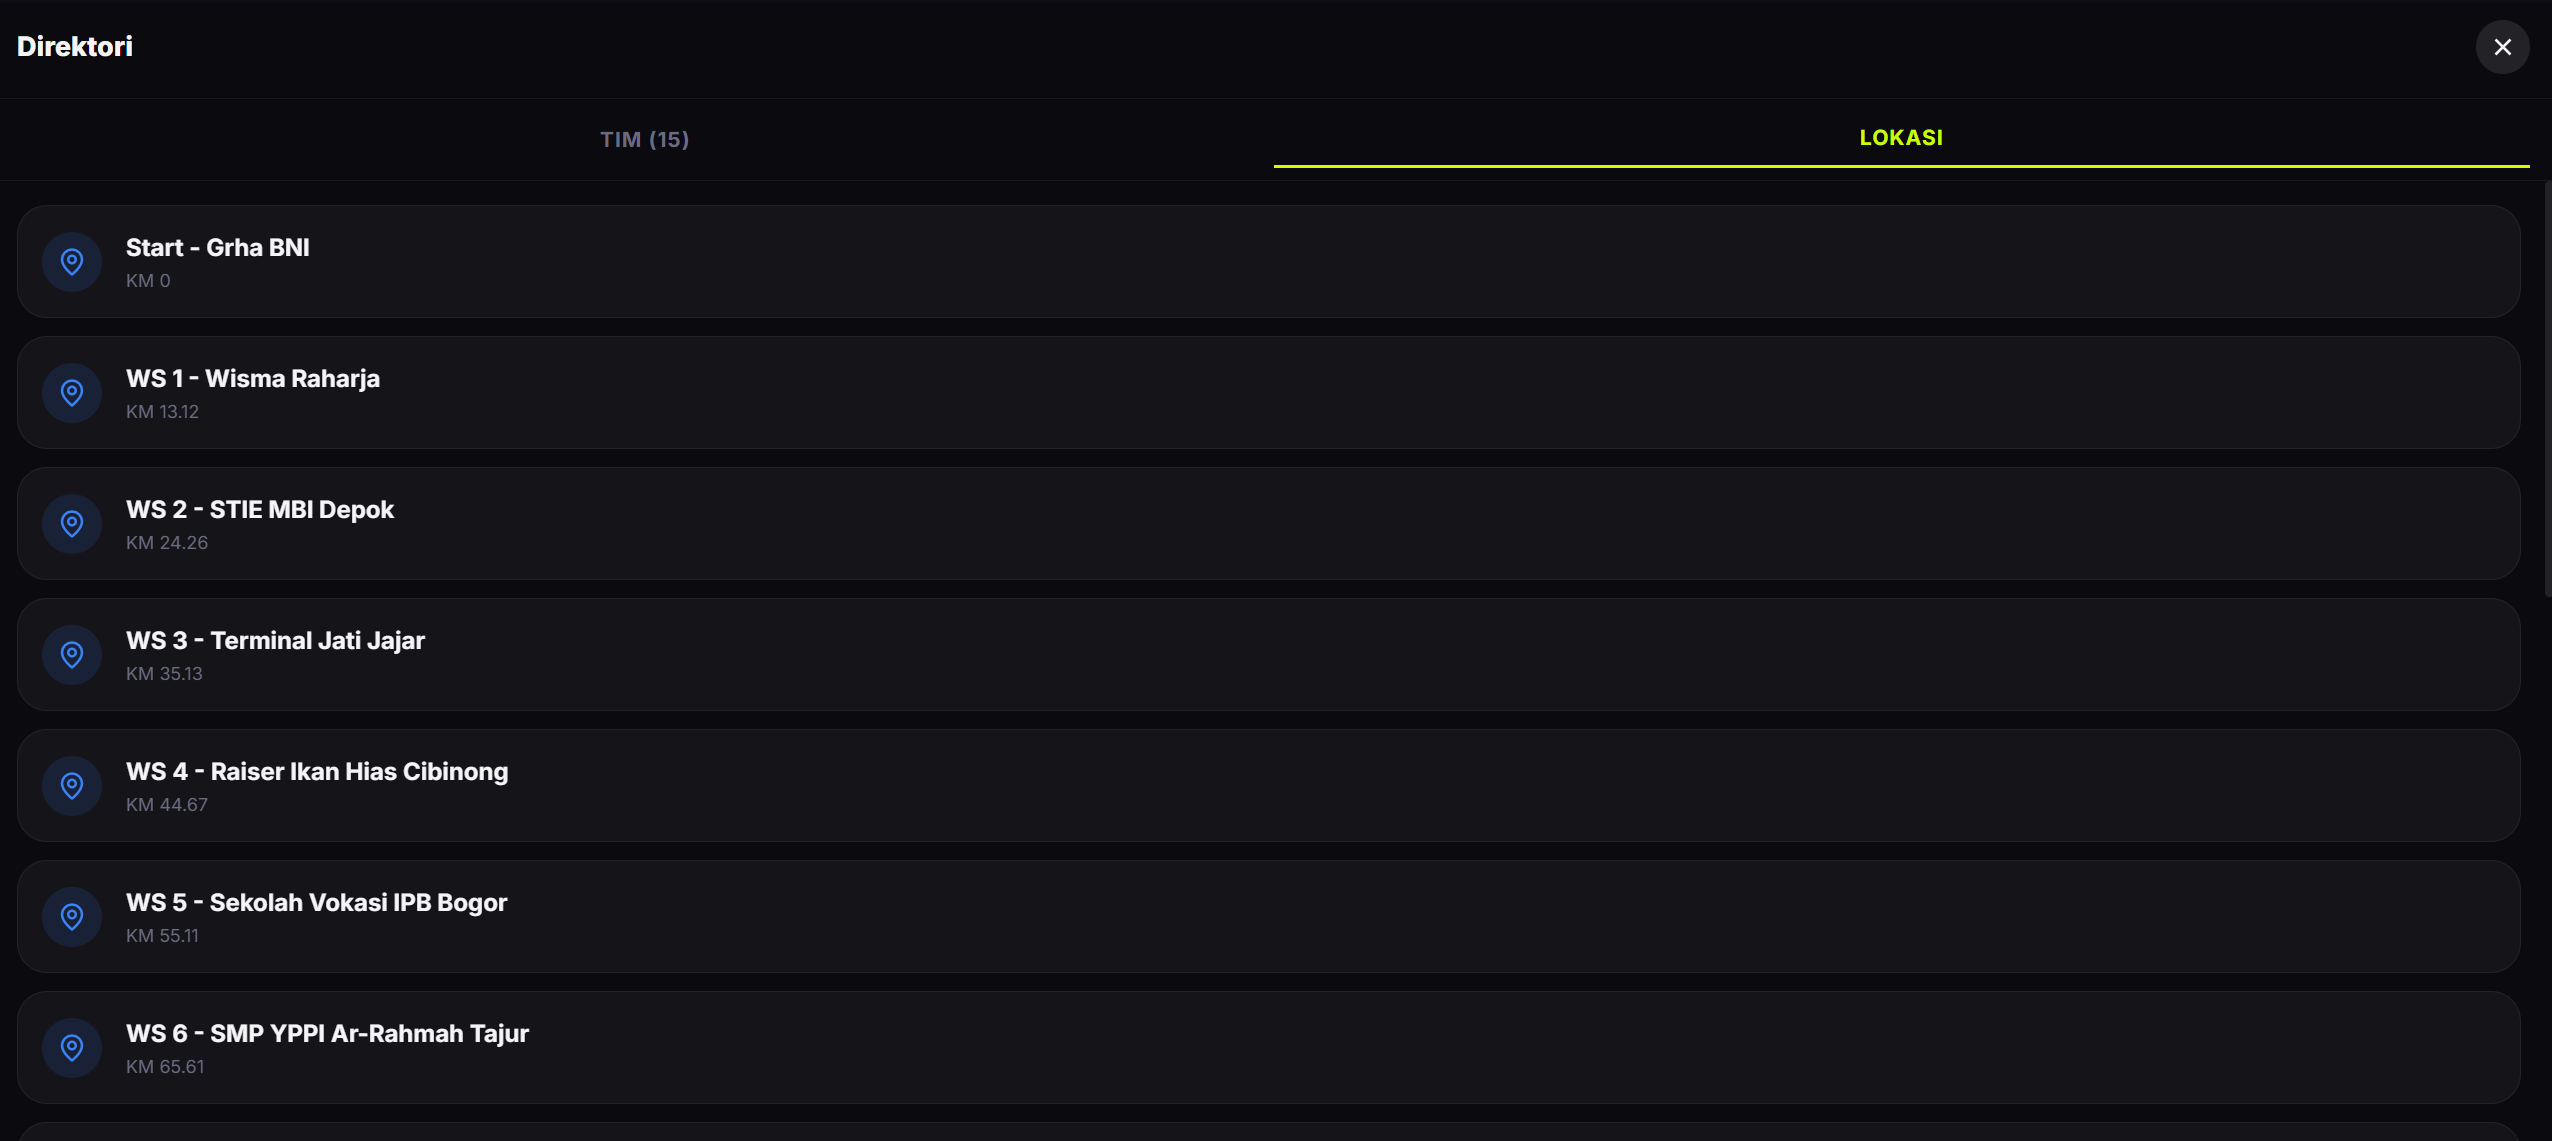
\includegraphics[width=0.62\textwidth,keepaspectratio]{images/implementasi/web/public-location.png} \\

\end{longtable}

% ============================================================
\section*{A.3 Aplikasi Web --- Halaman Ketua Tim}
\addcontentsline{toc}{section}{A.3 Aplikasi Web --- Halaman Ketua Tim}
% ============================================================

\begin{longtable}{|>{\raggedright\arraybackslash}p{3.8cm}|c|}
\caption*{Tabel A.3 Hasil Implementasi Antarmuka Web --- Halaman Ketua Tim} \\
\hline
\textbf{Fitur} & \textbf{Gambar} \\ \hline
\endfirsthead
\hline
\textbf{Fitur} & \textbf{Gambar} \\ \hline
\endhead
\hline
\endfoot
\hline
\endlastfoot

\textit{Dashboard} utama ketua tim yang menampilkan peta \textit{live} seluruh anggota tim beserta panel informasi &
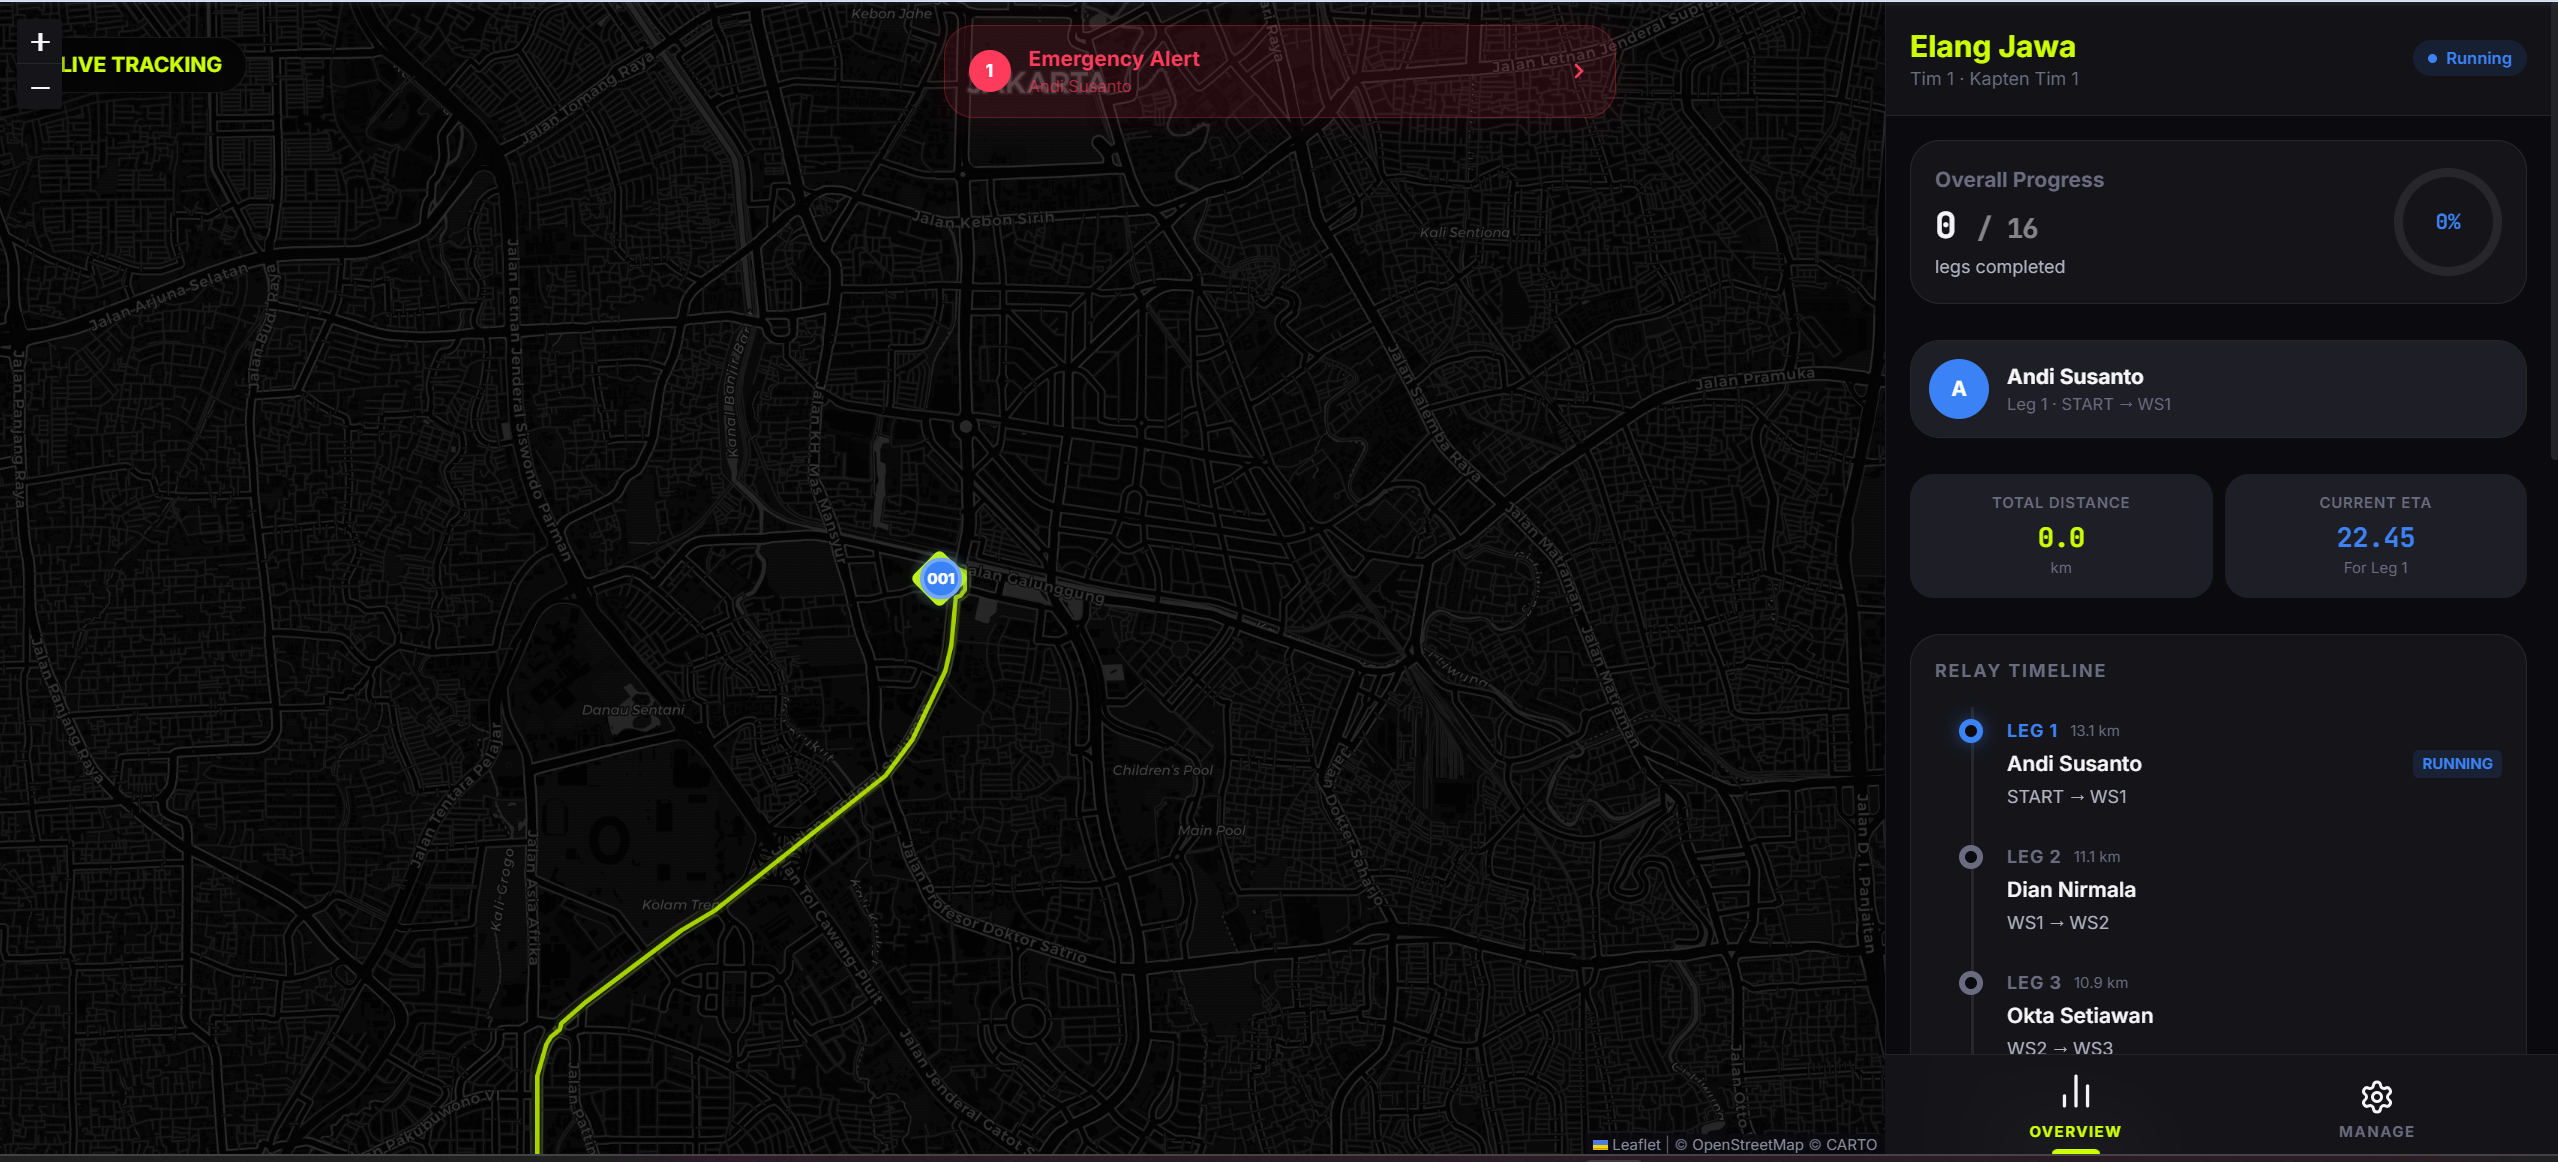
\includegraphics[width=0.62\textwidth,keepaspectratio]{images/implementasi/web/ketua-home.png} \\ \hline

Halaman manajemen tim untuk mengatur rotasi pelari dan membuat tautan untuk \textit{supporter} dan penonton &
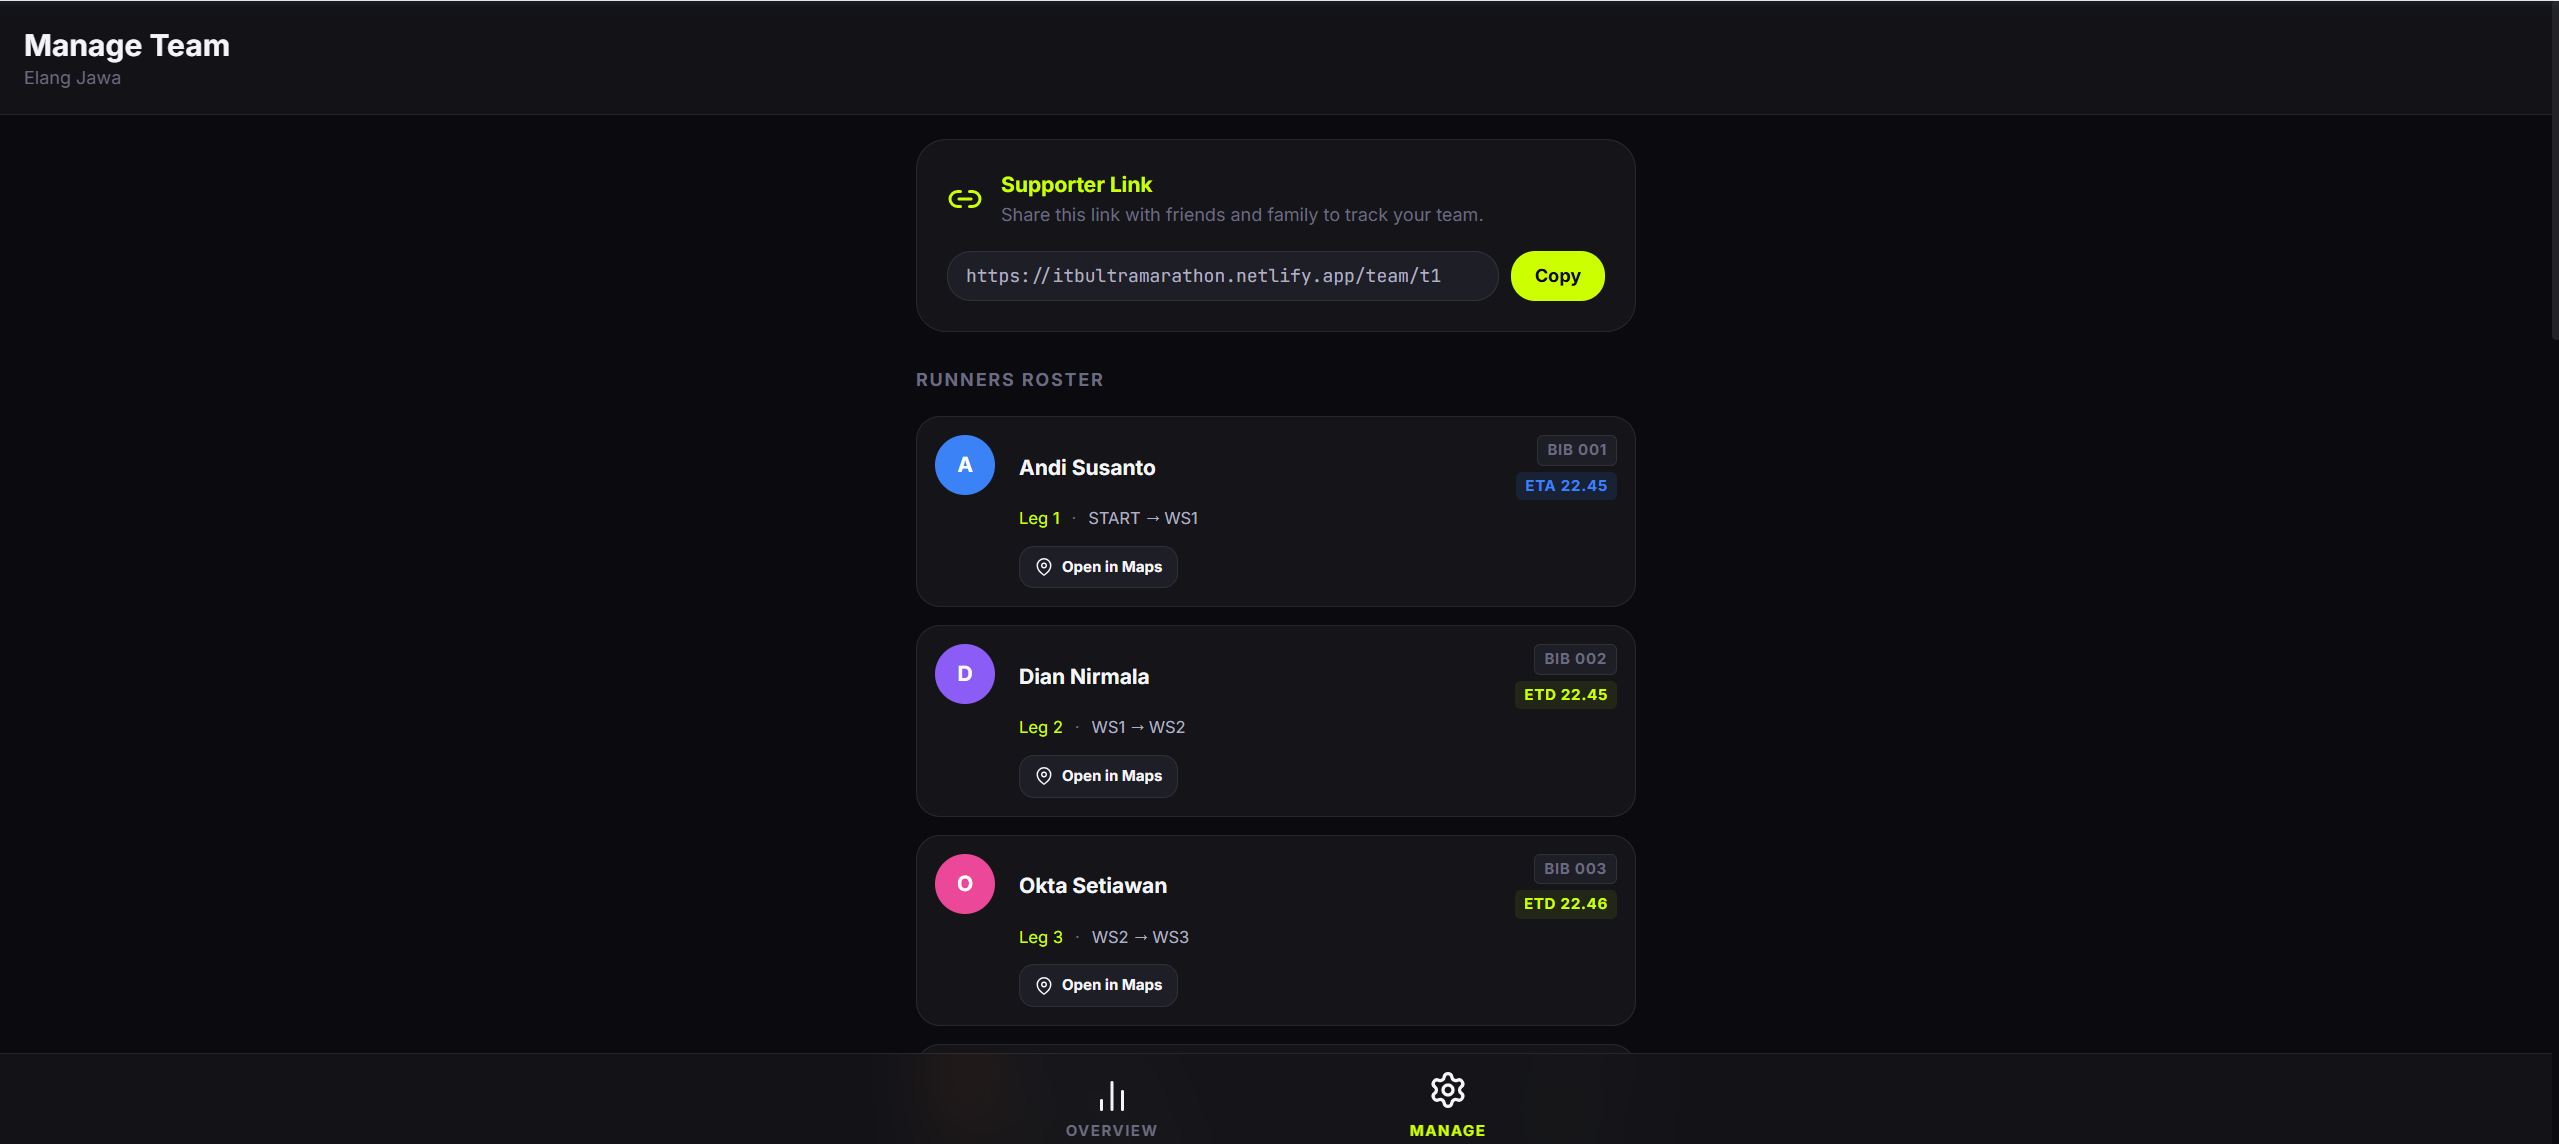
\includegraphics[width=0.62\textwidth,keepaspectratio]{images/implementasi/web/ketua-manage.png} \\

\end{longtable}

% ============================================================
\section*{A.4 Aplikasi Web --- Halaman Supporter}
\addcontentsline{toc}{section}{A.4 Aplikasi Web --- Halaman Supporter}
% ============================================================

\begin{longtable}{|>{\raggedright\arraybackslash}p{3.8cm}|c|}
\caption*{Tabel A.4 Hasil Implementasi Antarmuka Web --- Halaman Supporter} \\
\hline
\textbf{Fitur} & \textbf{Gambar} \\ \hline
\endfirsthead
\hline
\textbf{Fitur} & \textbf{Gambar} \\ \hline
\endhead
\hline
\endfoot
\hline
\endlastfoot

\textit{Dashboard} utama \textit{supporter} yang menampilkan peta dan posisi pelari yang sedang dipantau secara \textit{real-time} &
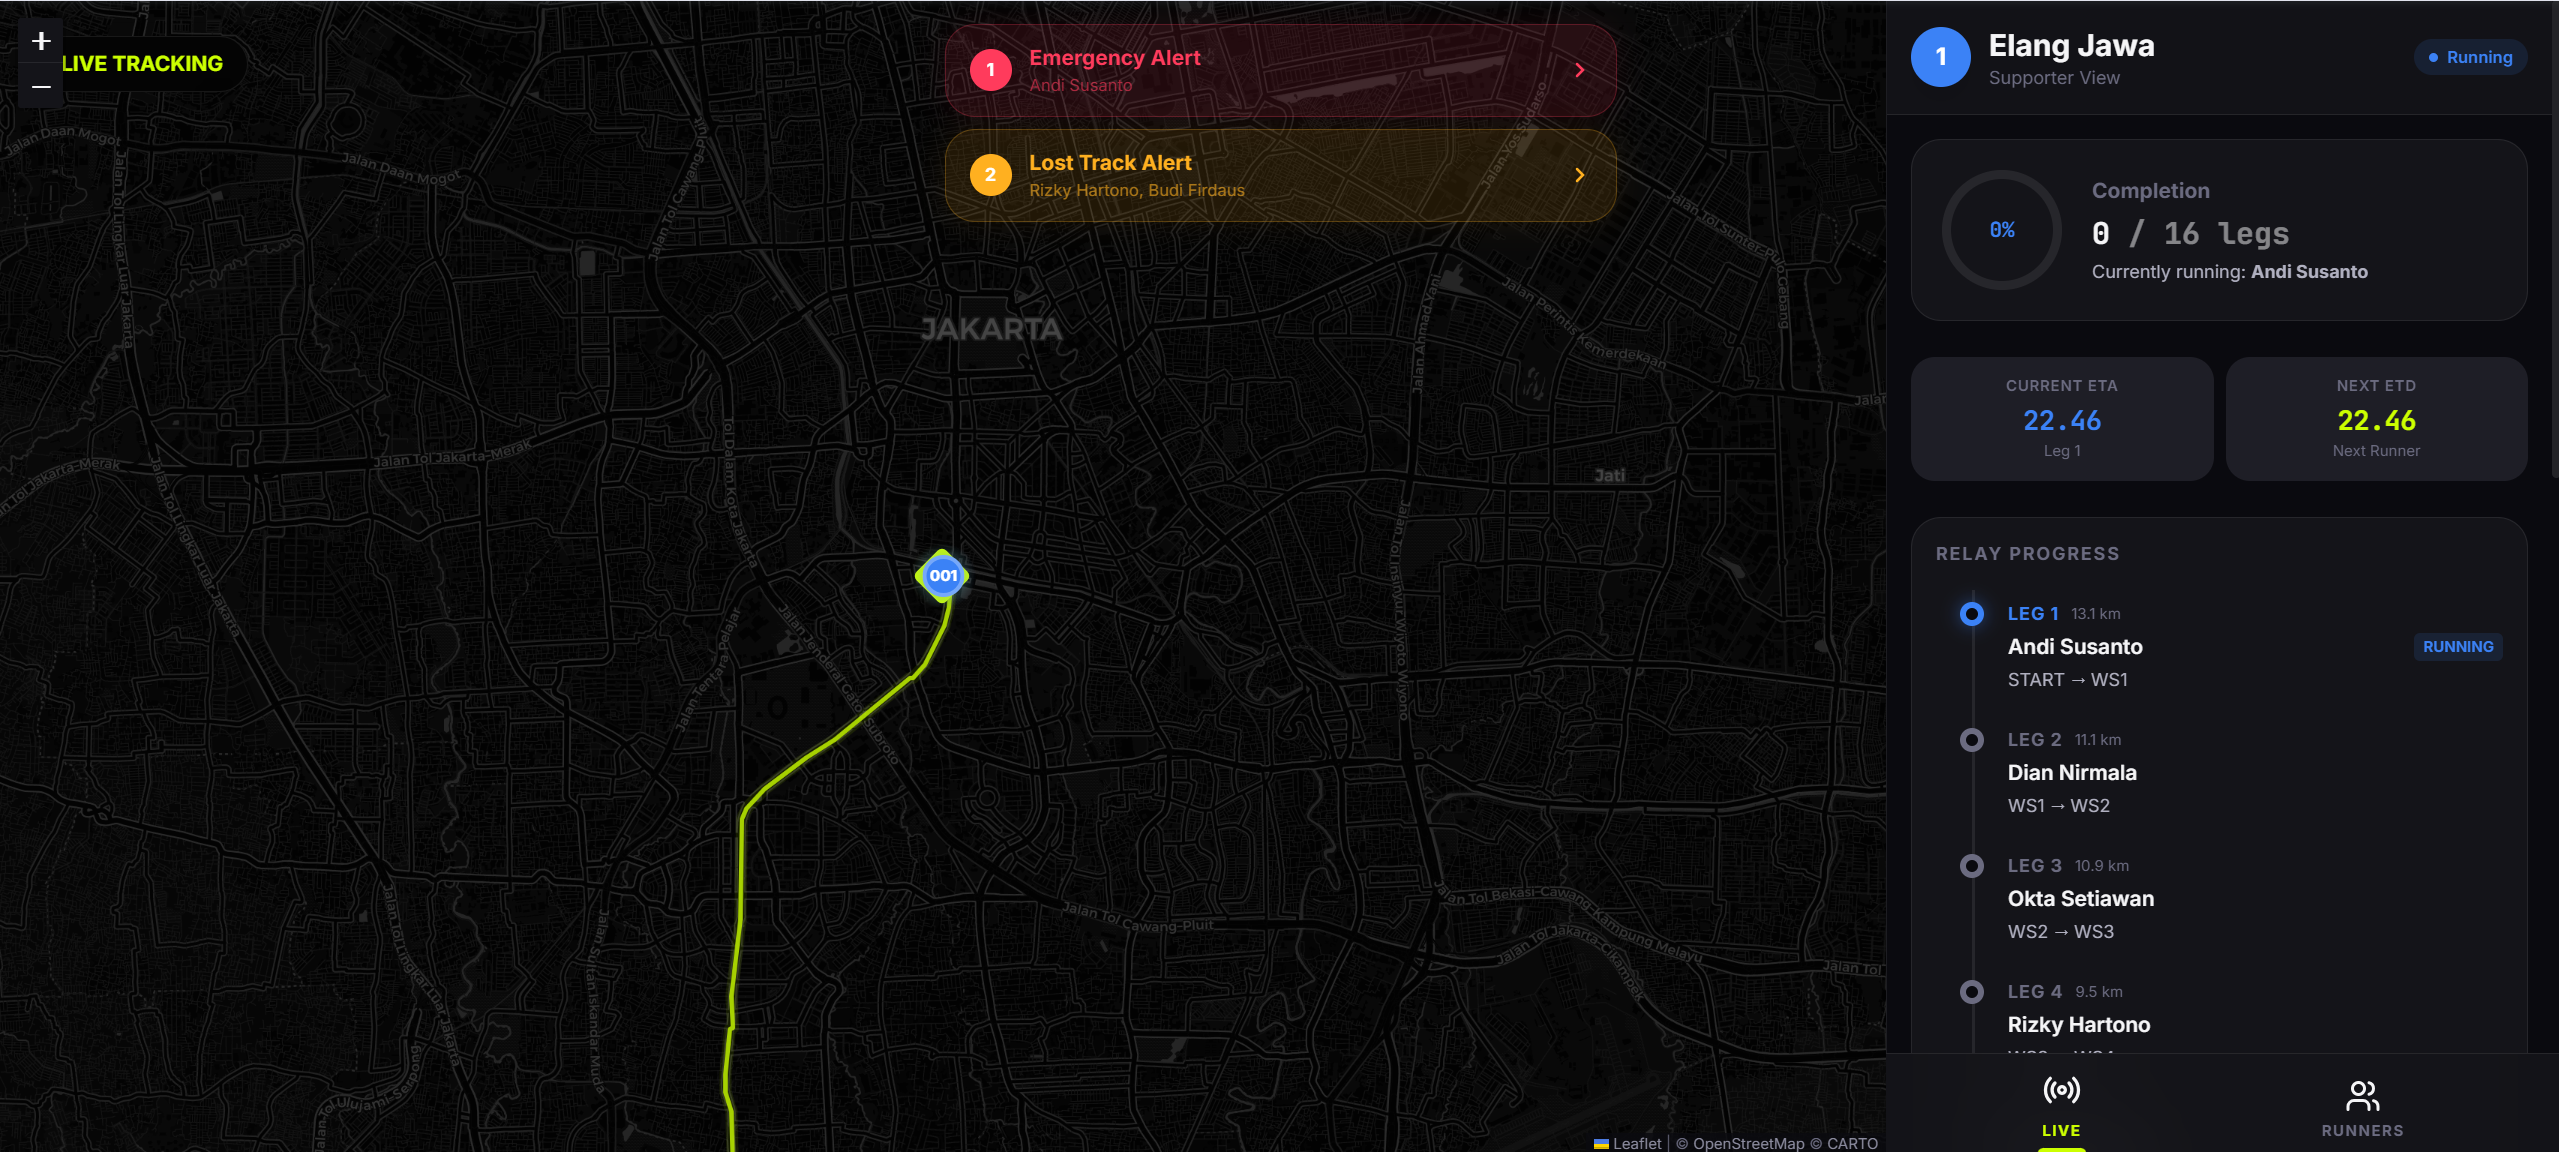
\includegraphics[width=0.62\textwidth,keepaspectratio]{images/implementasi/web/support-home.png} \\ \hline

Halaman manajemen \textit{supporter} untuk memilih peserta yang dipantau dan mengakses navigasi ke lokasi pelari &
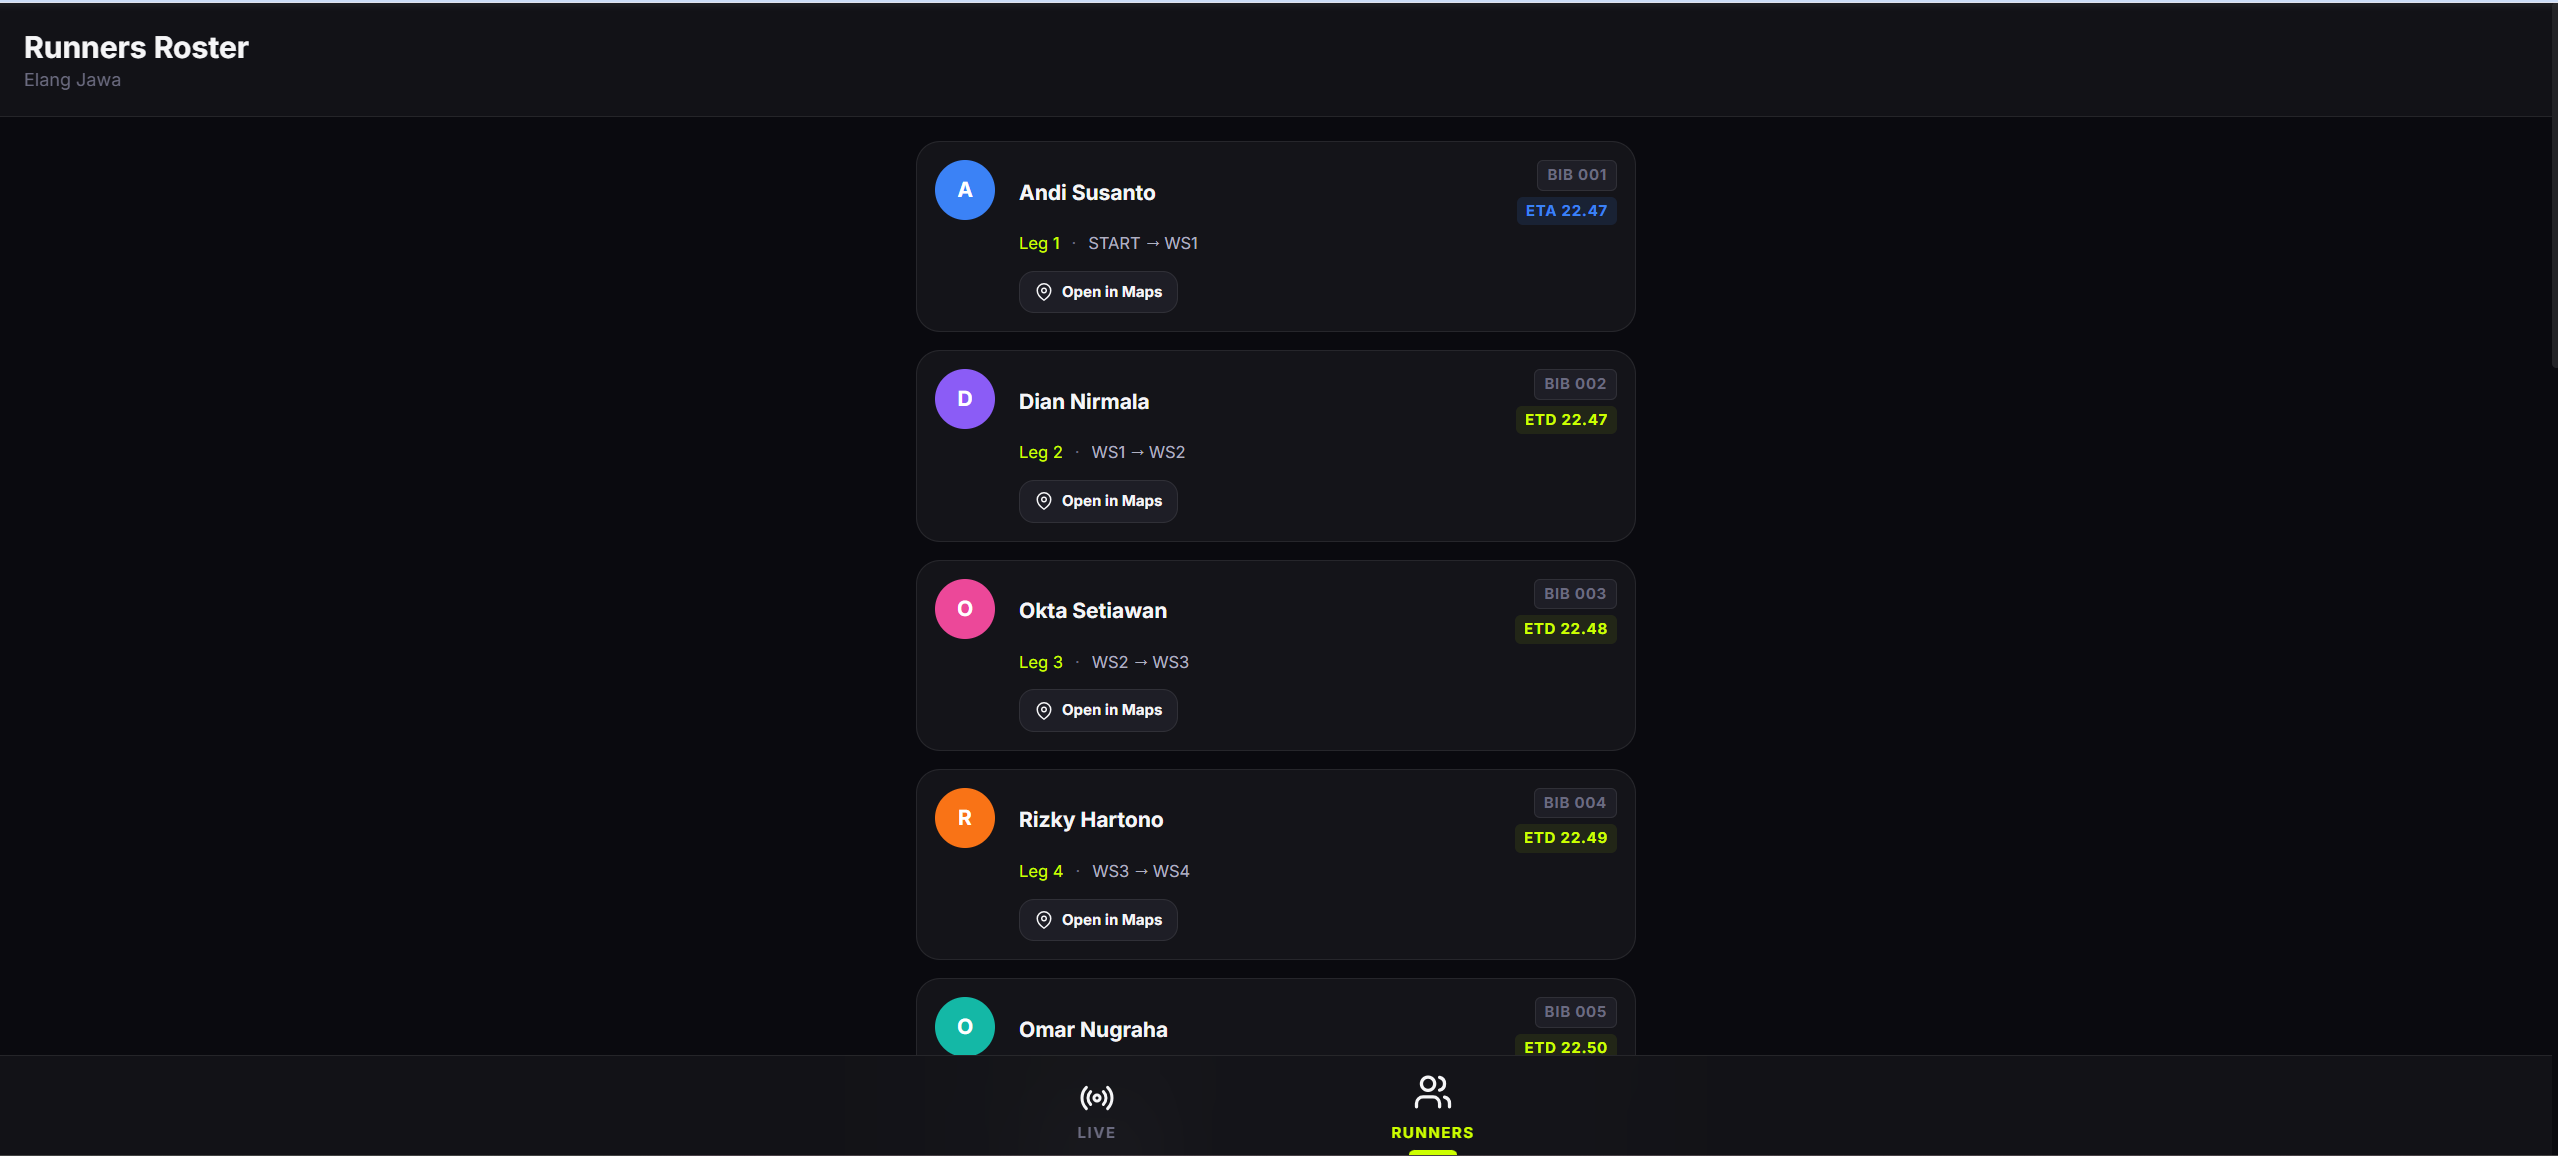
\includegraphics[width=0.62\textwidth,keepaspectratio]{images/implementasi/web/support-manage.png} \\

\end{longtable}

% ============================================================
\section*{A.5 Aplikasi Web --- Halaman Panitia}
\addcontentsline{toc}{section}{A.5 Aplikasi Web --- Halaman Panitia}
% ============================================================

\begin{longtable}{|>{\raggedright\arraybackslash}p{3.8cm}|c|}
\caption*{Tabel A.5 Hasil Implementasi Antarmuka Web --- Halaman Panitia} \\
\hline
\textbf{Fitur} & \textbf{Gambar} \\ \hline
\endfirsthead
\hline
\textbf{Fitur} & \textbf{Gambar} \\ \hline
\endhead
\hline
\endfoot
\hline
\endlastfoot

\textit{Dashboard} statistik perlombaan yang merangkum data keseluruhan seperti jumlah tim aktif dan pelari selesai &
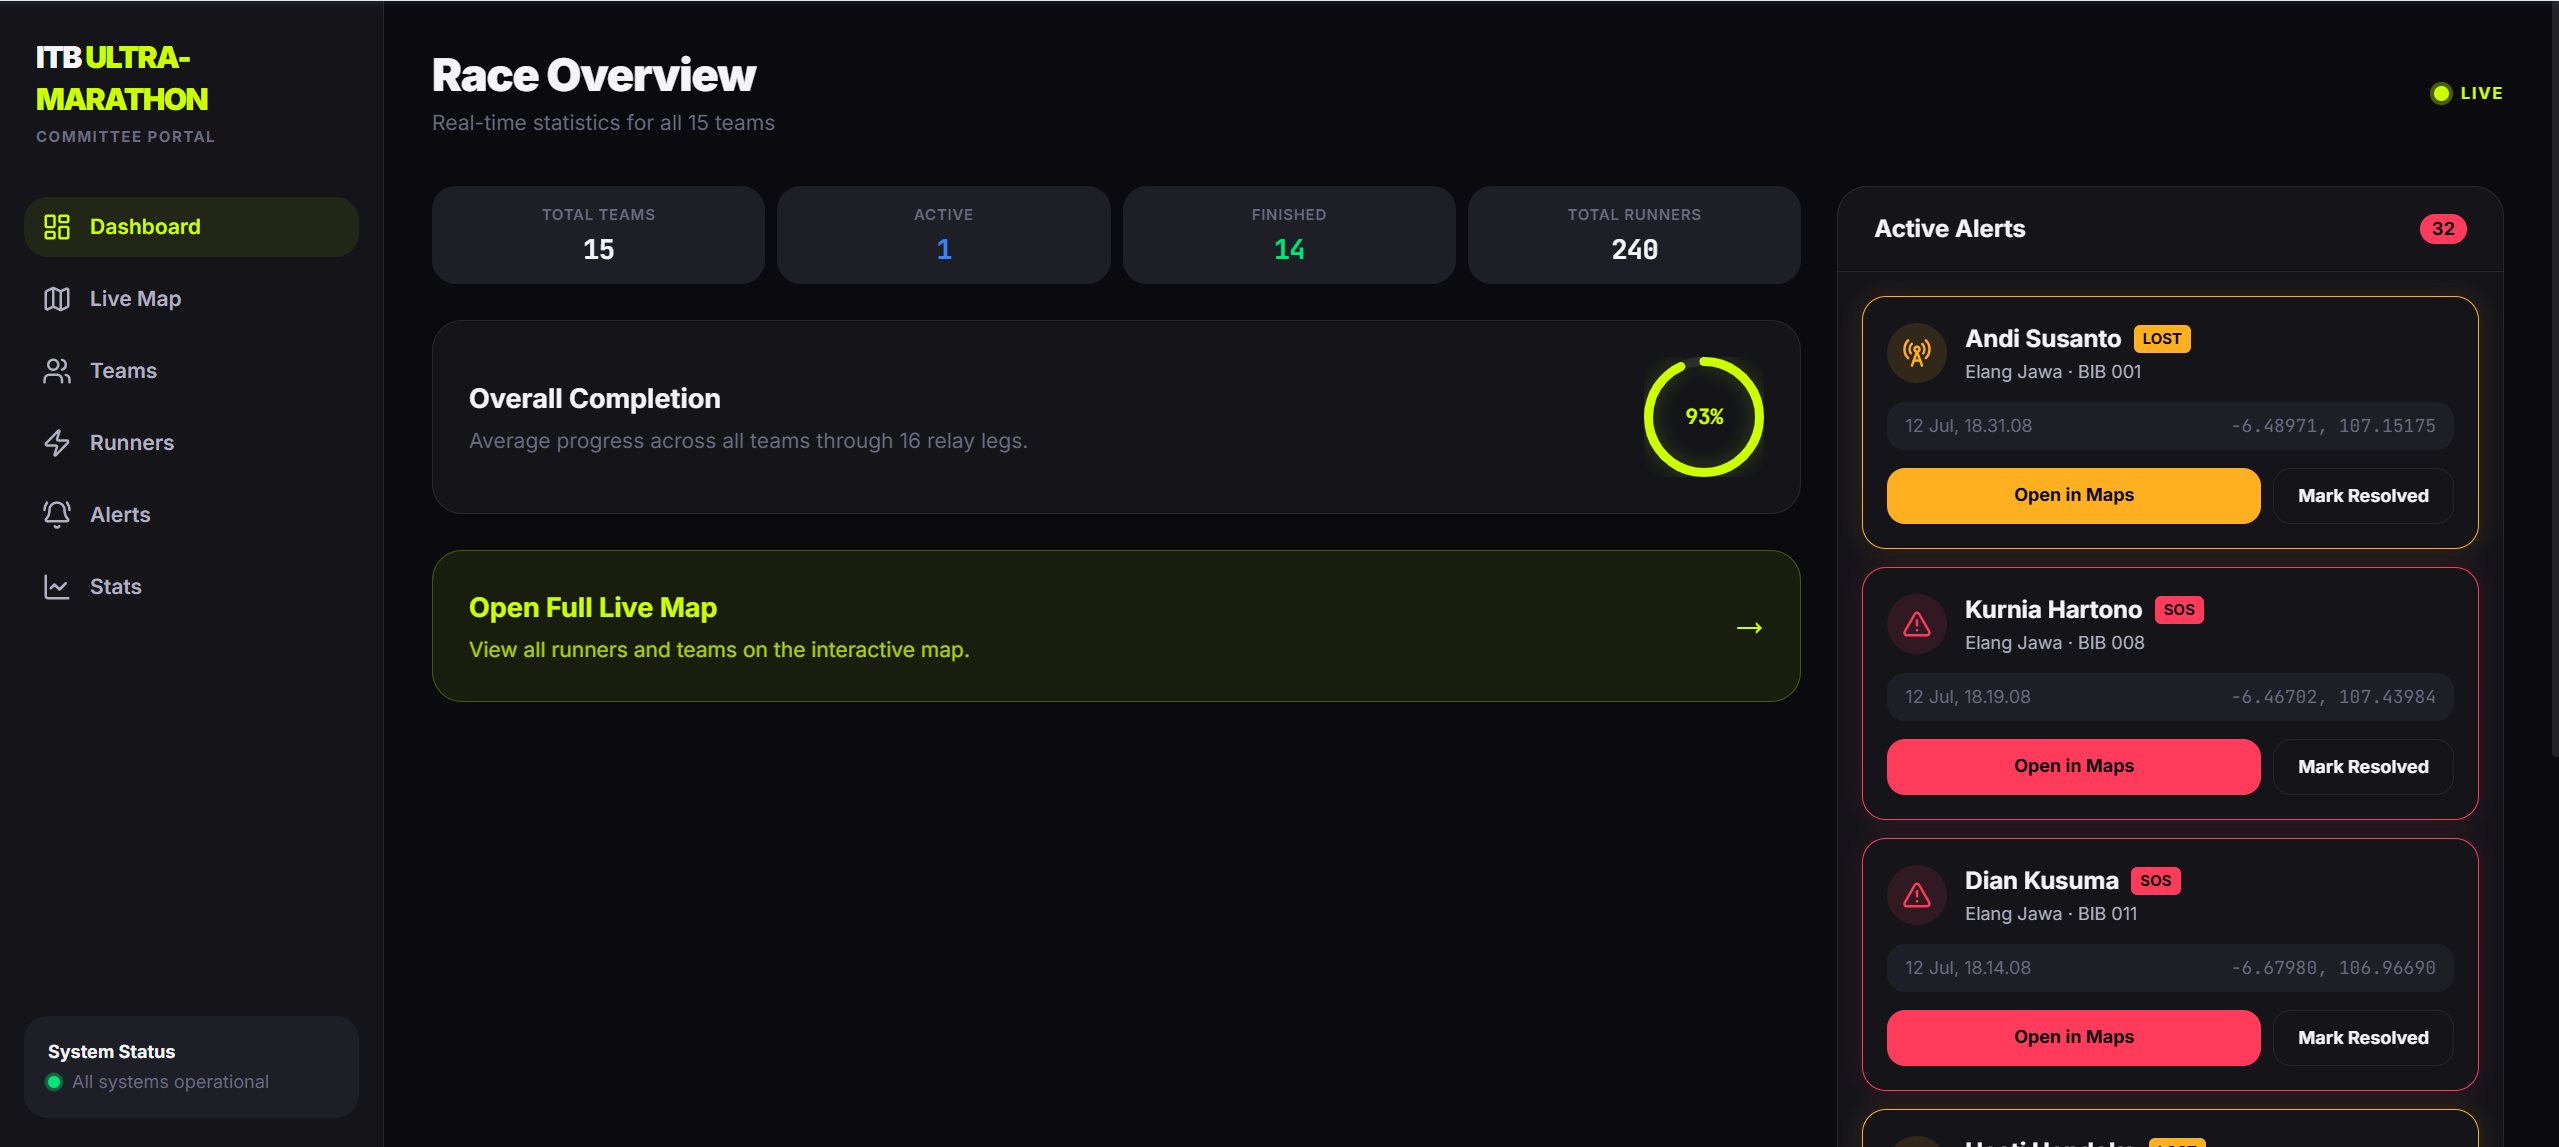
\includegraphics[width=0.62\textwidth,keepaspectratio]{images/implementasi/web/panitia-dasahboard.png} \\ \hline

Tampilan peta global yang memperlihatkan posisi seluruh pelari dari semua tim secara bersamaan &
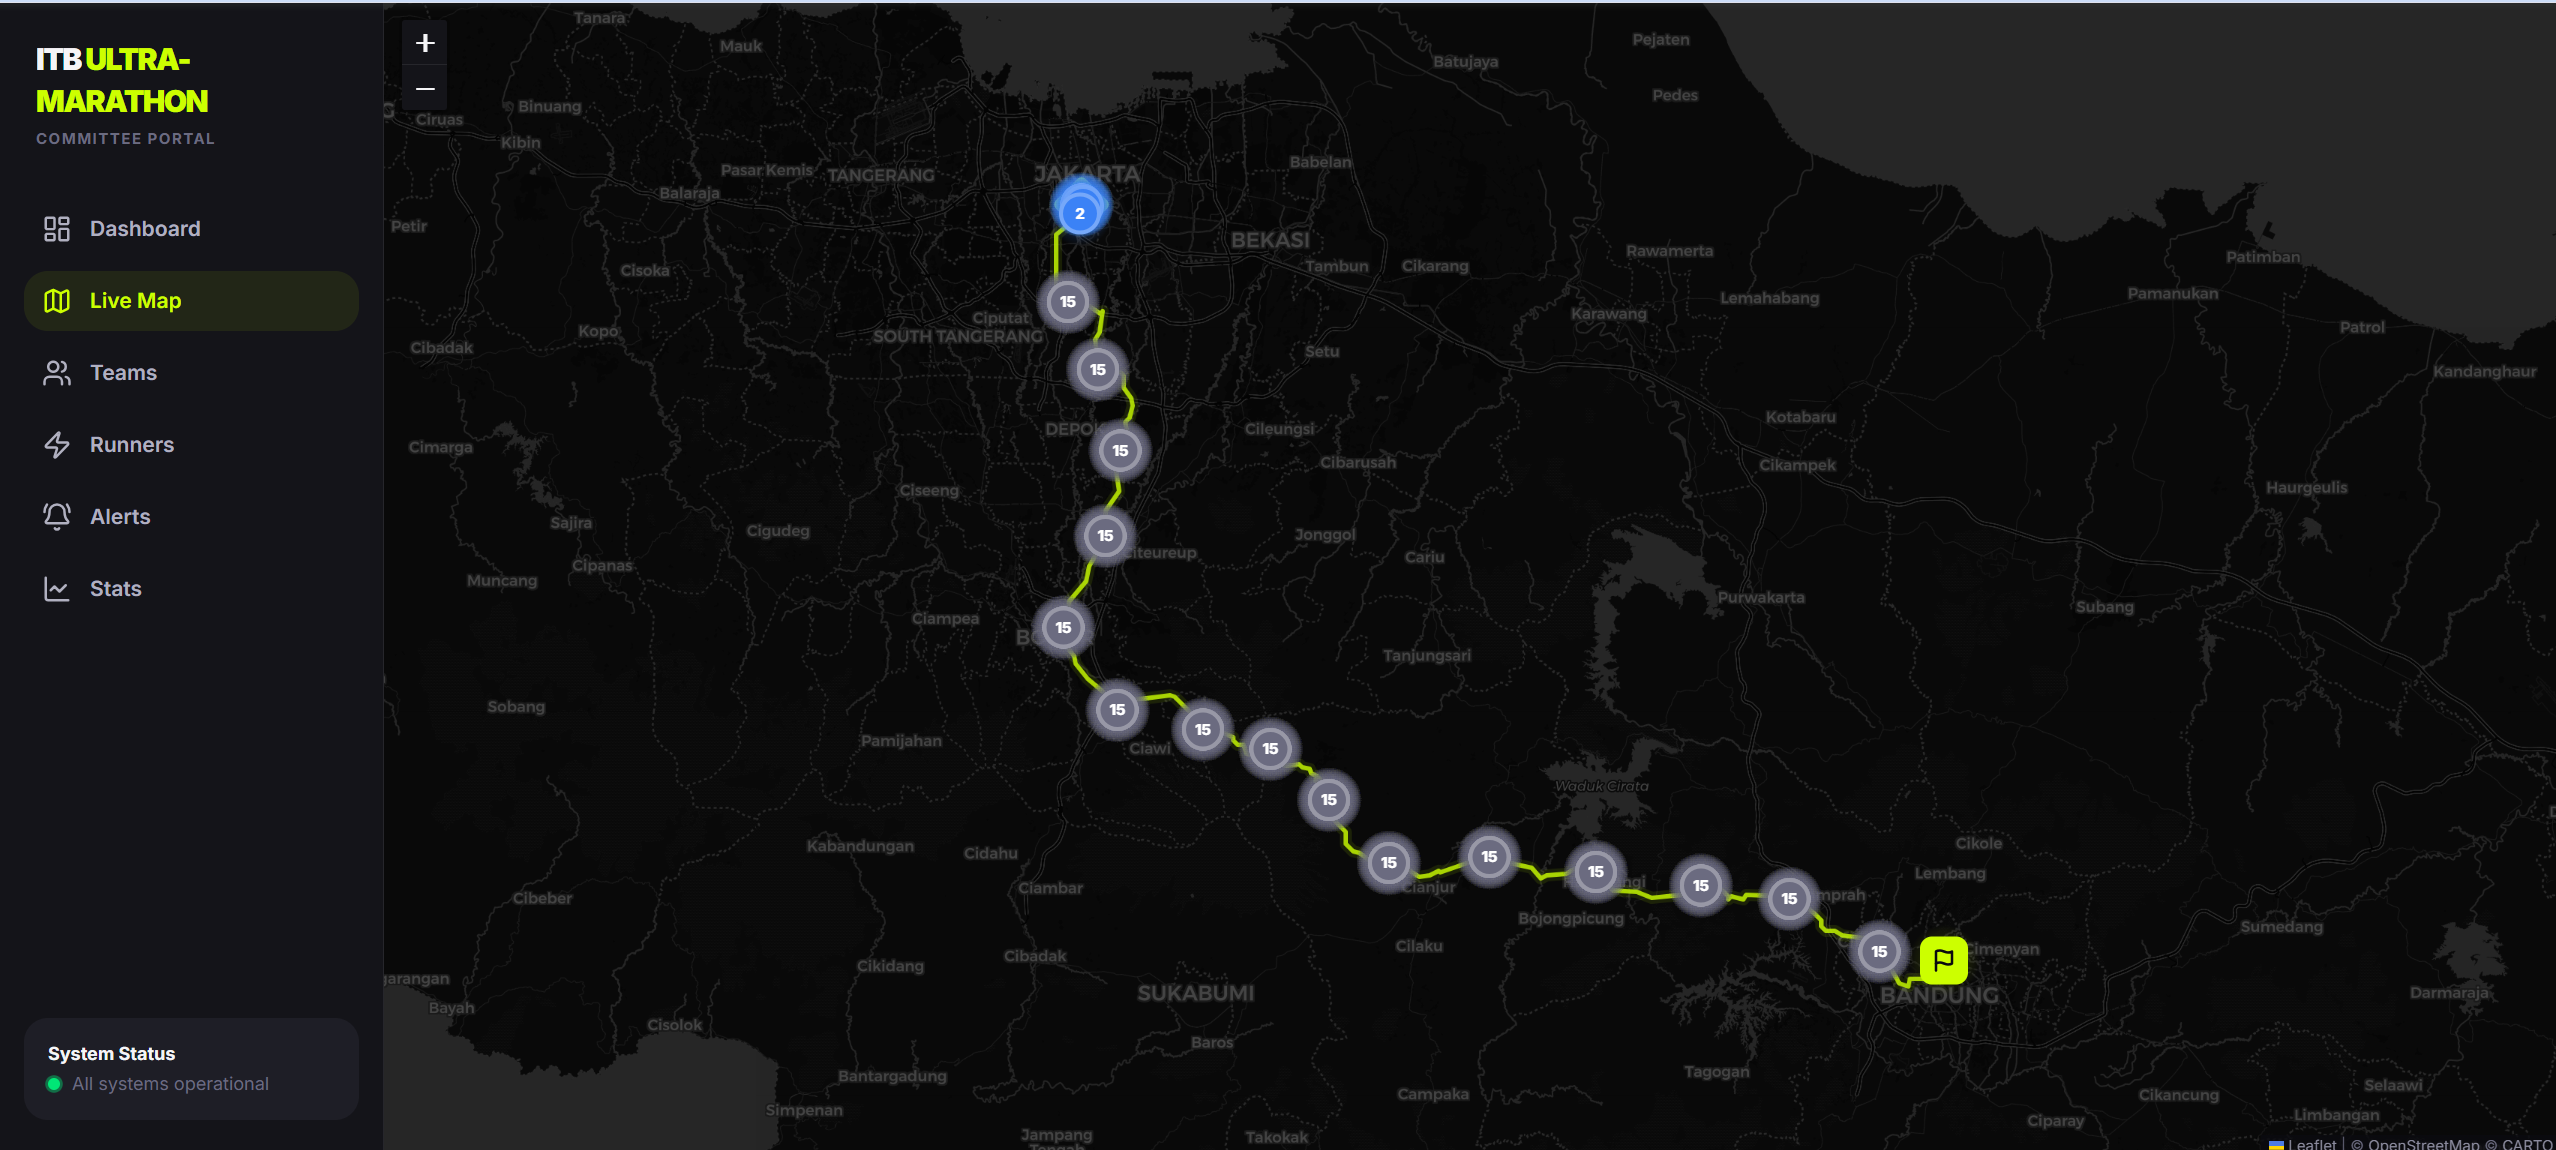
\includegraphics[width=0.62\textwidth,keepaspectratio]{images/implementasi/web/panitia-map.png} \\ \hline

Halaman \textit{command center} darurat yang menampilkan peringatan SOS berkedip beserta koordinat pelari &
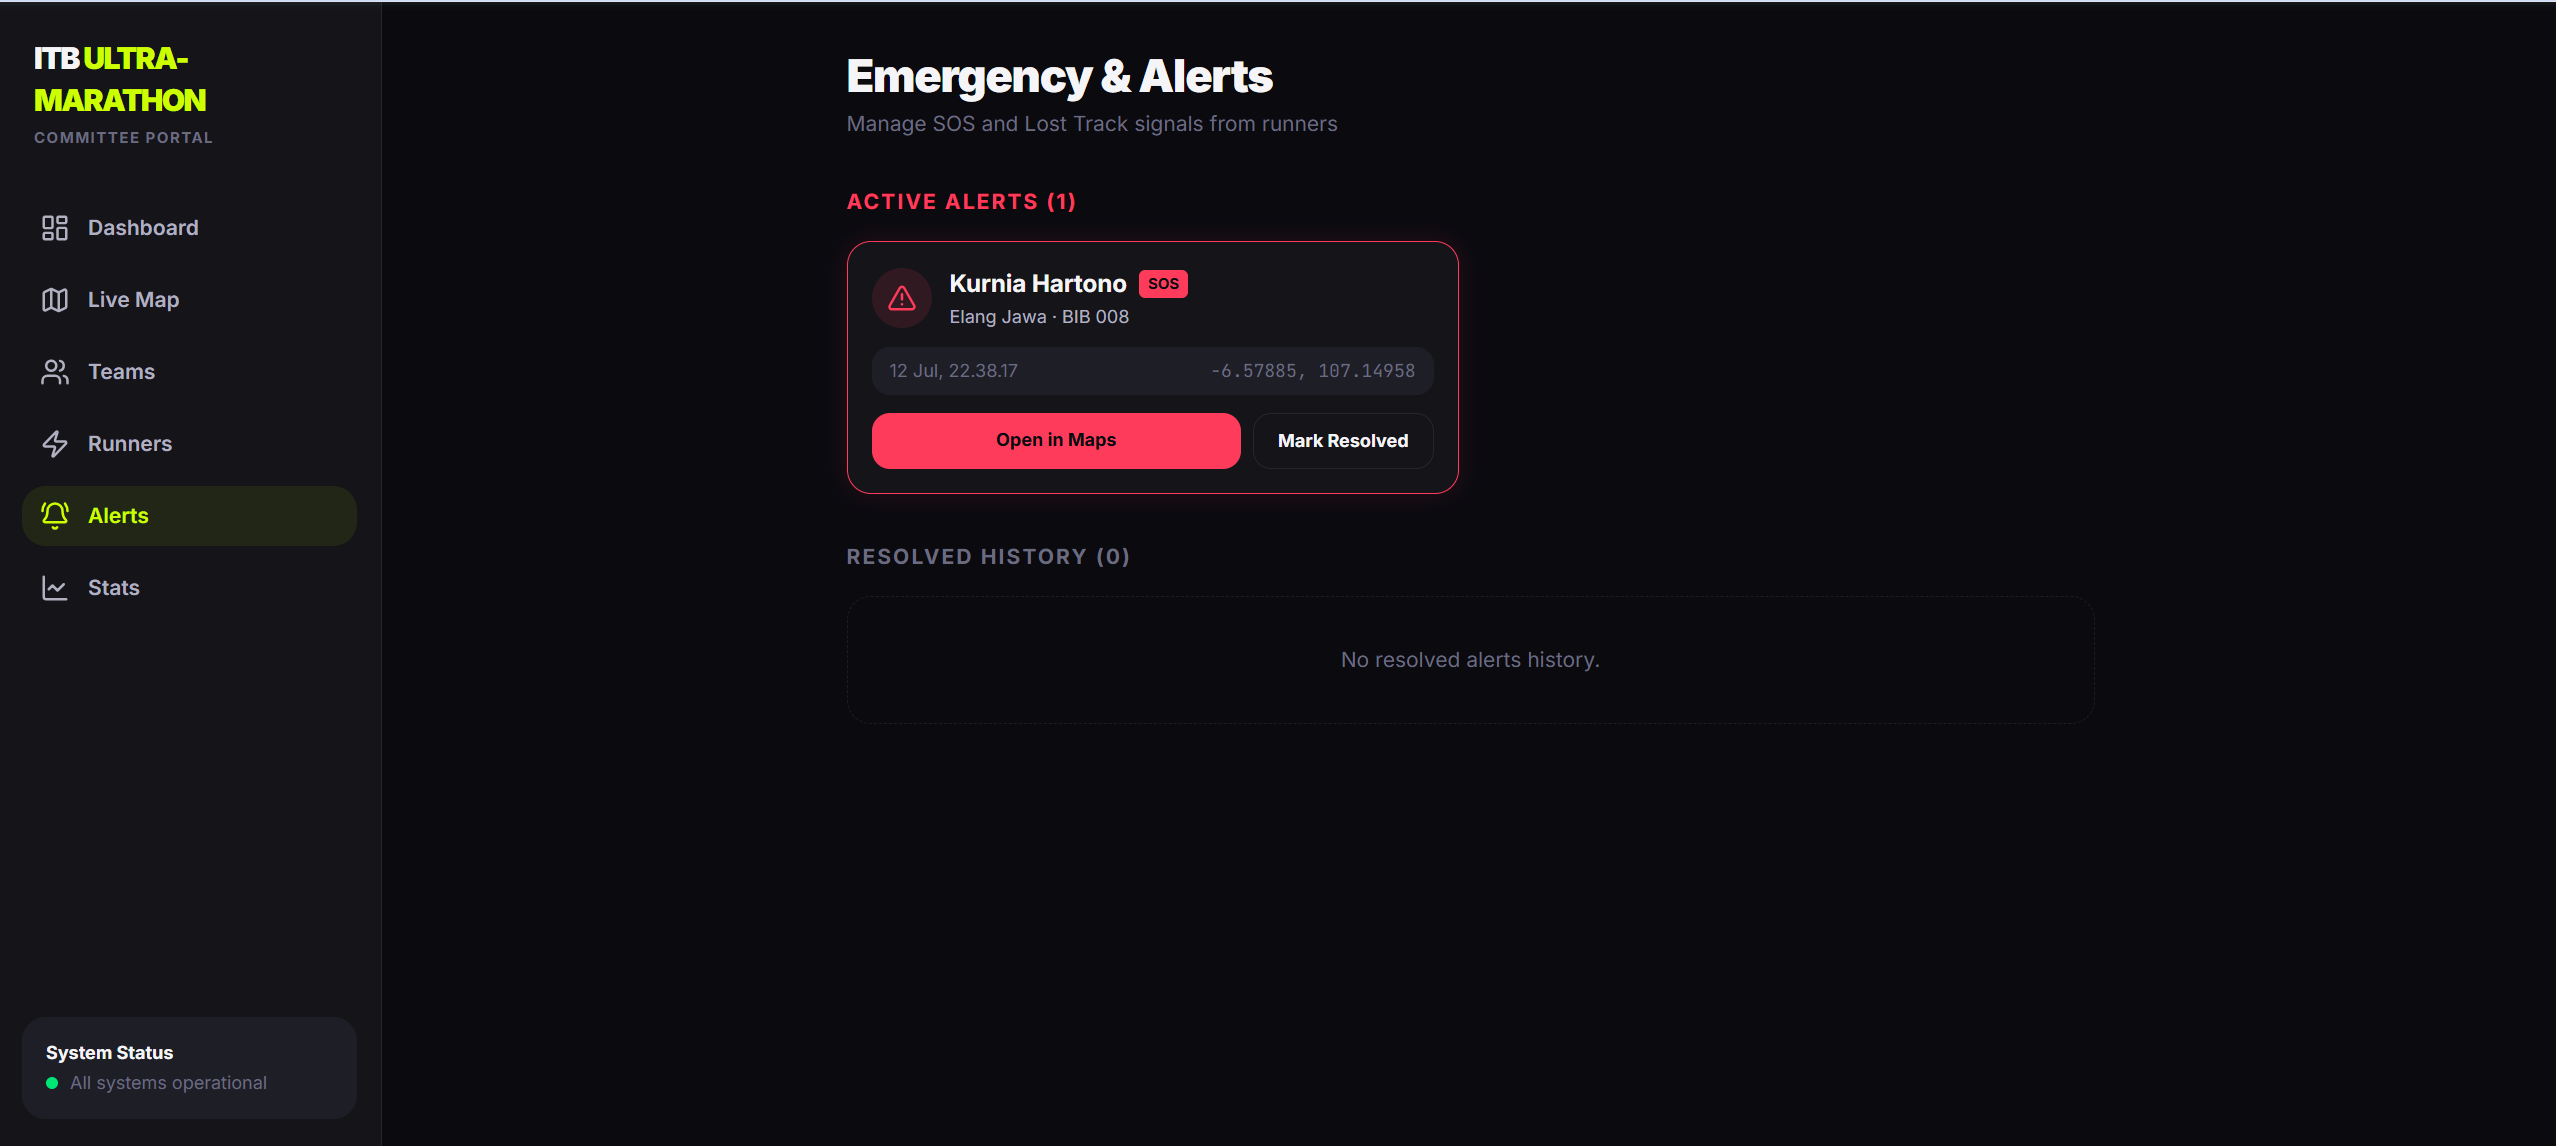
\includegraphics[width=0.62\textwidth,keepaspectratio]{images/implementasi/web/panitia-alert.png} \\ \hline

Halaman daftar pelari yang menampilkan status seluruh peserta perlombaan secara terpusat &
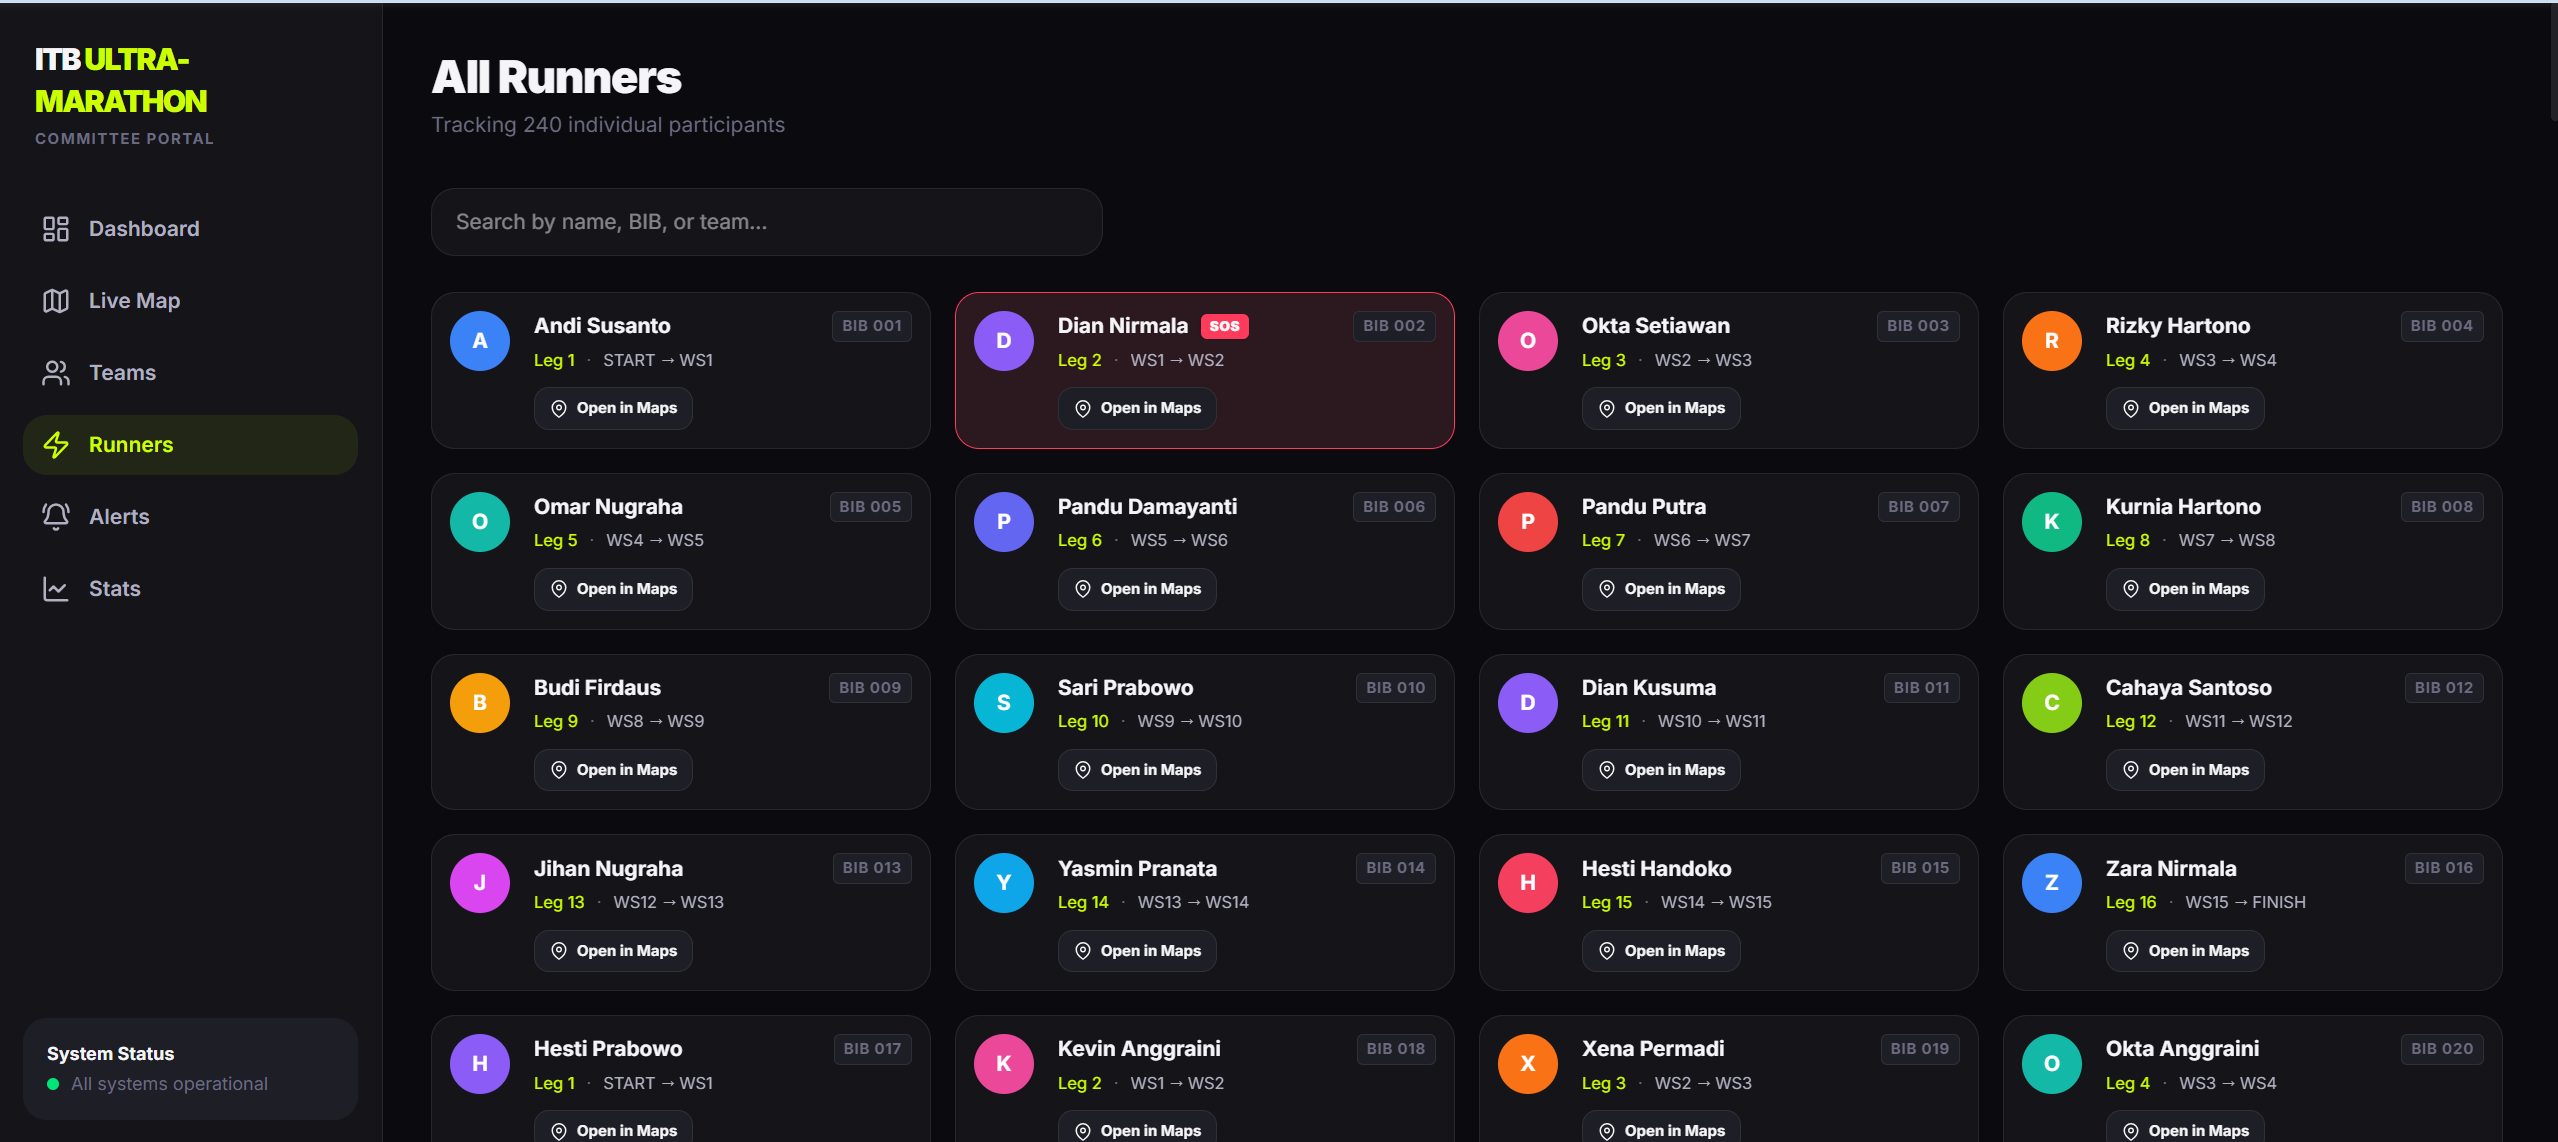
\includegraphics[width=0.62\textwidth,keepaspectratio]{images/implementasi/web/panitia-runner.png} \\ \hline

Halaman daftar tim yang menampilkan informasi dan susunan anggota dari setiap tim yang terdaftar &
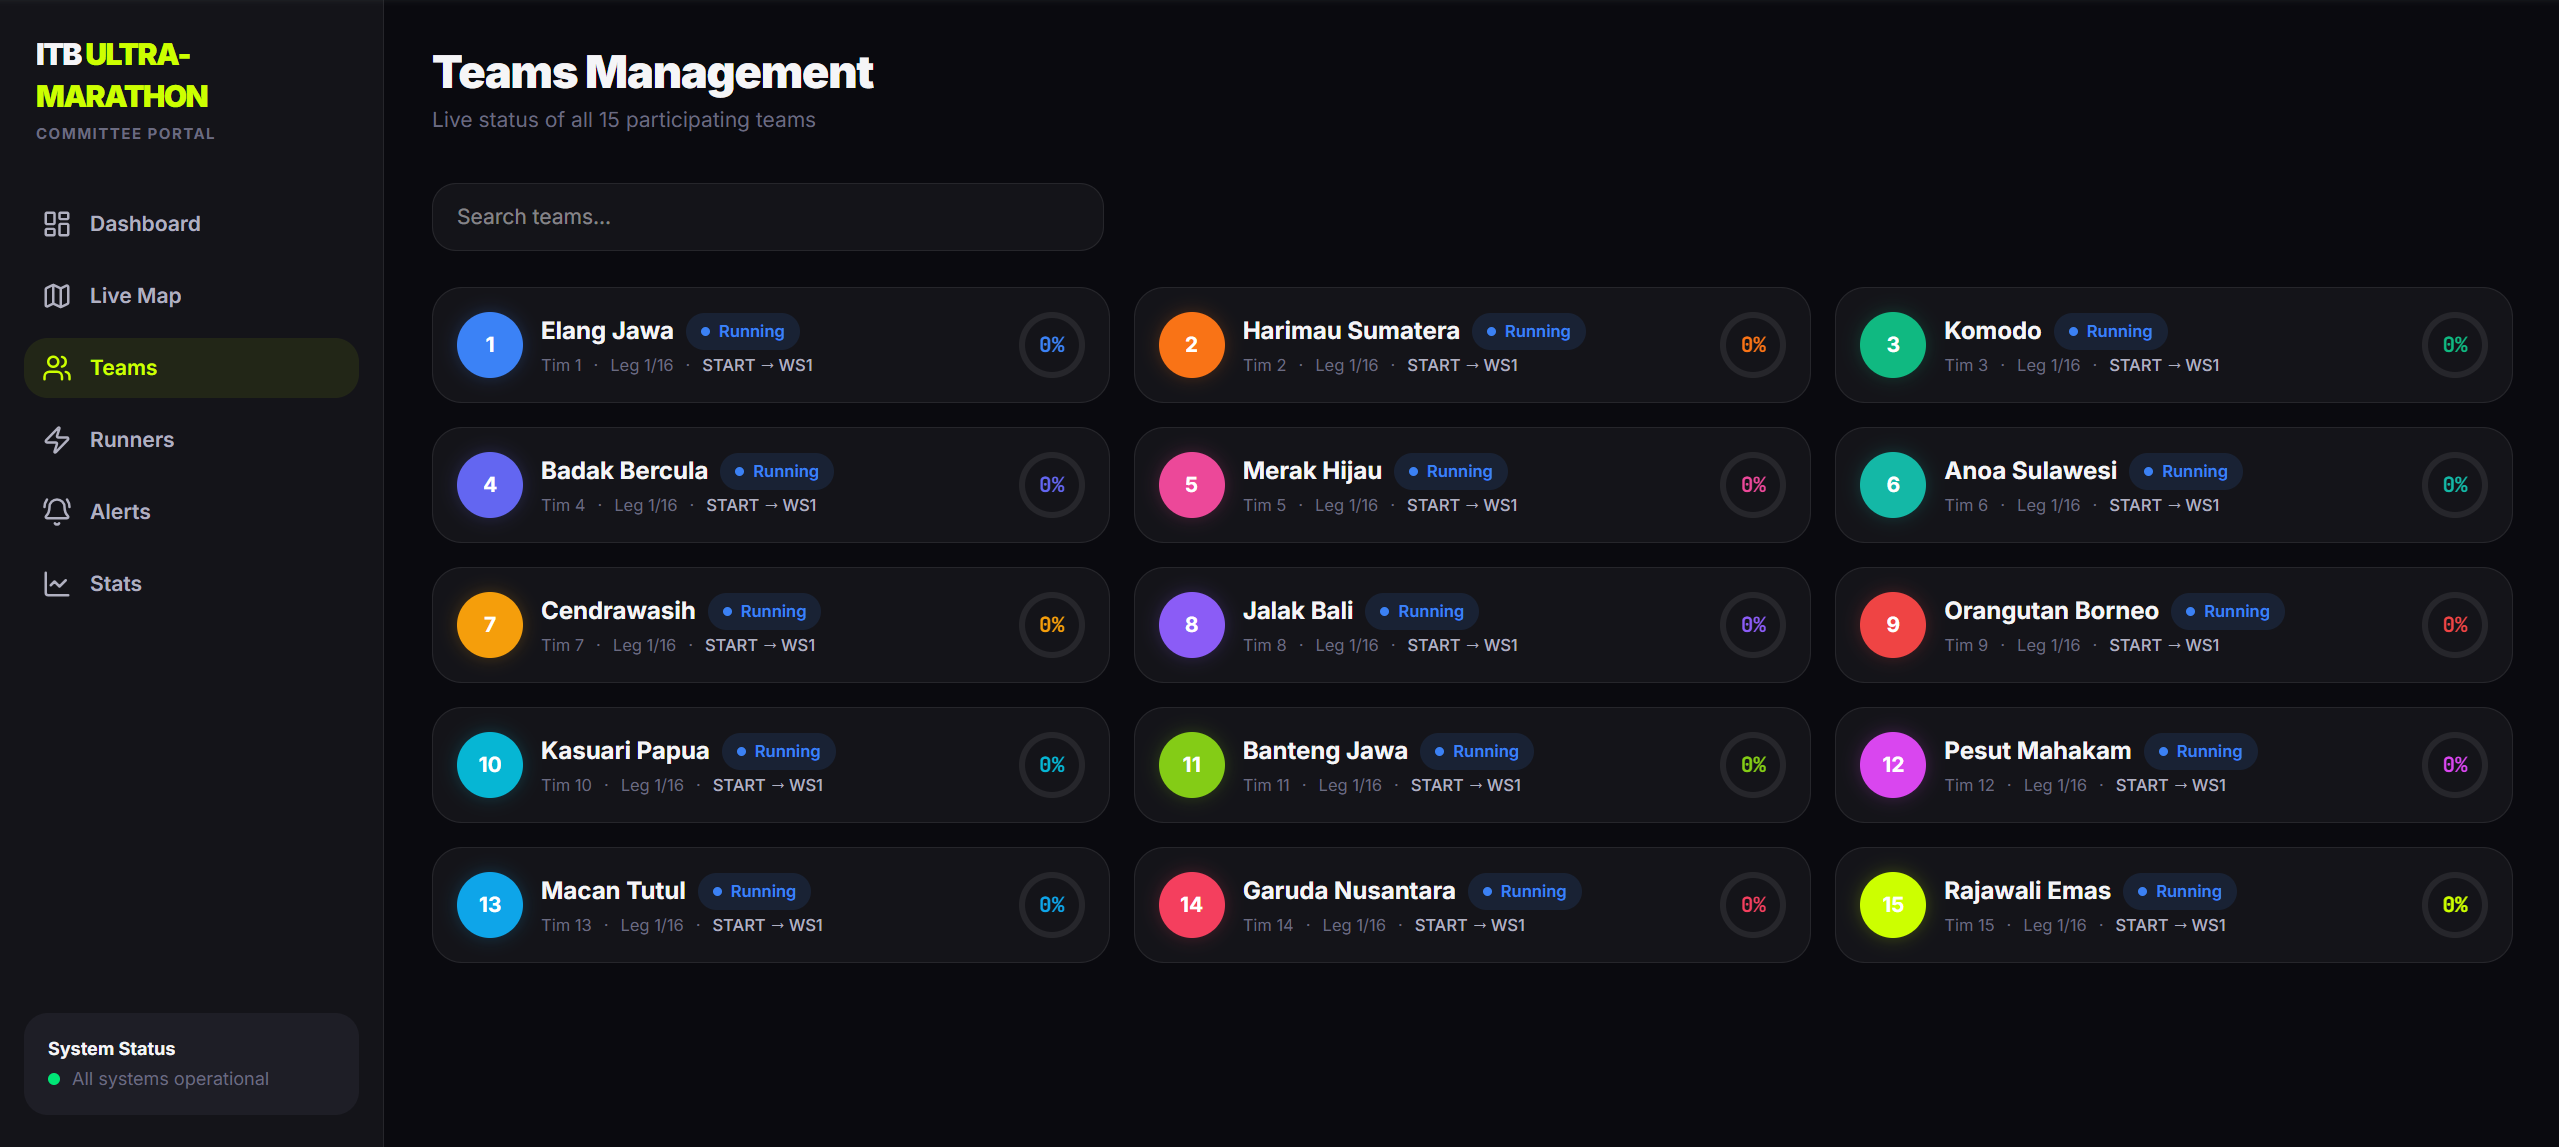
\includegraphics[width=0.62\textwidth,keepaspectratio]{images/implementasi/web/panitia-team.png} \\ \hline

Halaman statistik perlombaan yang menampilkan rekapitulasi performa perlombaan secara \textit{real-time} &
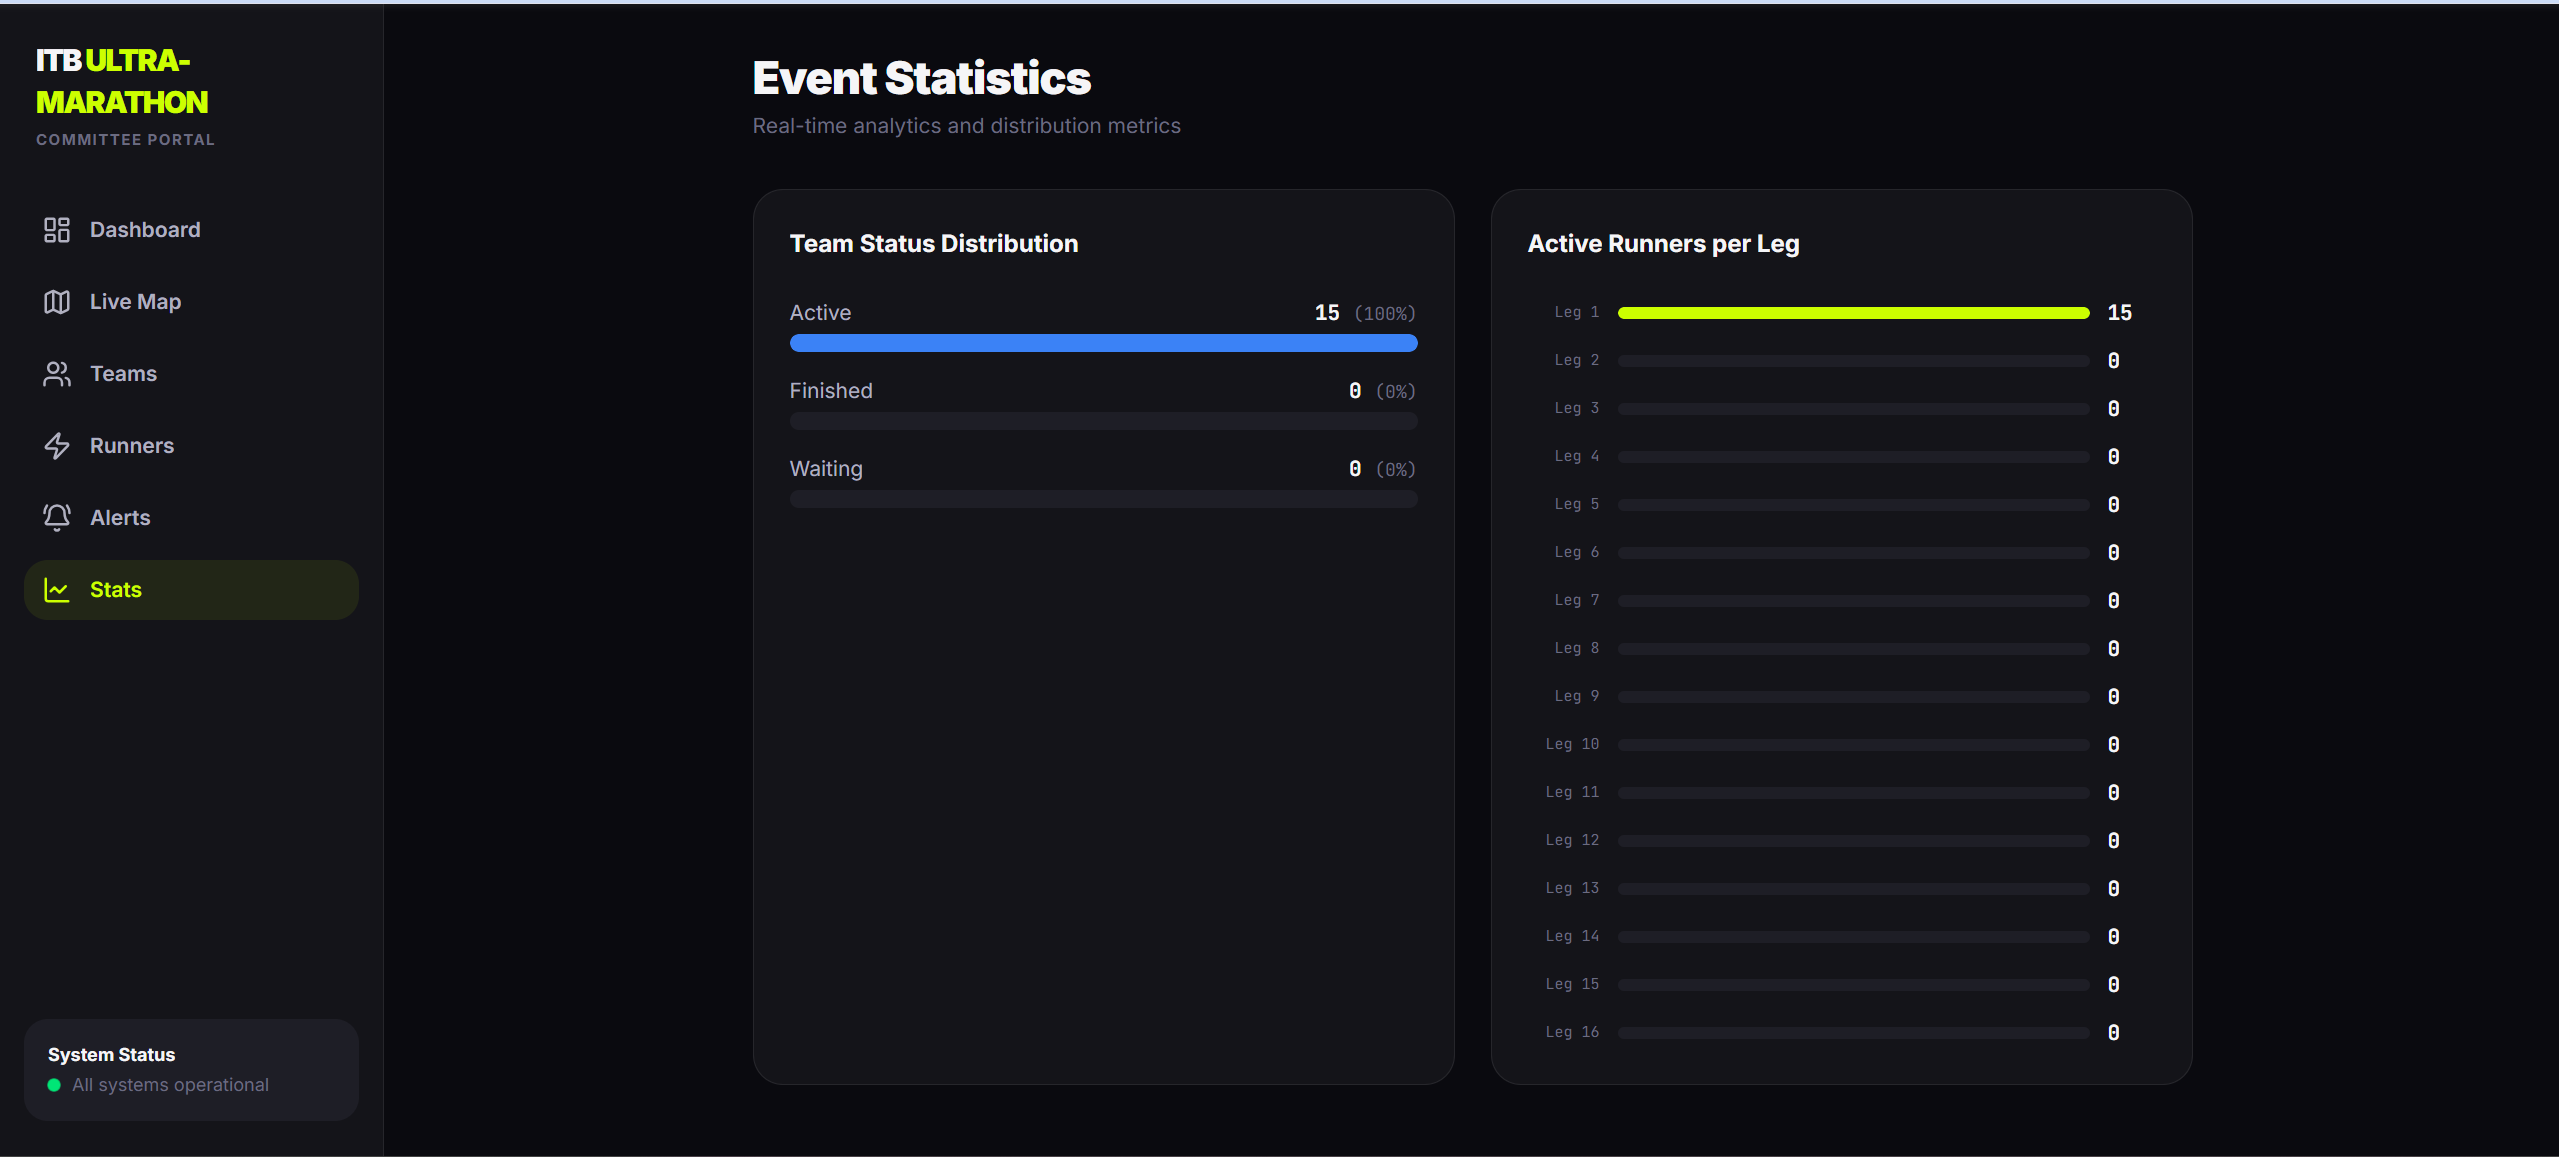
\includegraphics[width=0.62\textwidth,keepaspectratio]{images/implementasi/web/panitia-stats.png} \\

\end{longtable}

% ============================================================
\section*{A.6 Aplikasi Web --- Halaman Penonton}
\addcontentsline{toc}{section}{A.6 Aplikasi Web --- Halaman Penonton}
% ============================================================

\begin{longtable}{|>{\raggedright\arraybackslash}p{3.8cm}|c|}
\caption*{Tabel A.6 Hasil Implementasi Antarmuka Web --- Halaman Penonton} \\
\hline
\textbf{Fitur} & \textbf{Gambar} \\ \hline
\endfirsthead
\hline
\textbf{Fitur} & \textbf{Gambar} \\ \hline
\endhead
\hline
\endfoot
\hline
\endlastfoot

Halaman penonton (\textit{private view}) dengan kamera peta yang terkunci mengikuti posisi pelari yang sedang dipantau &
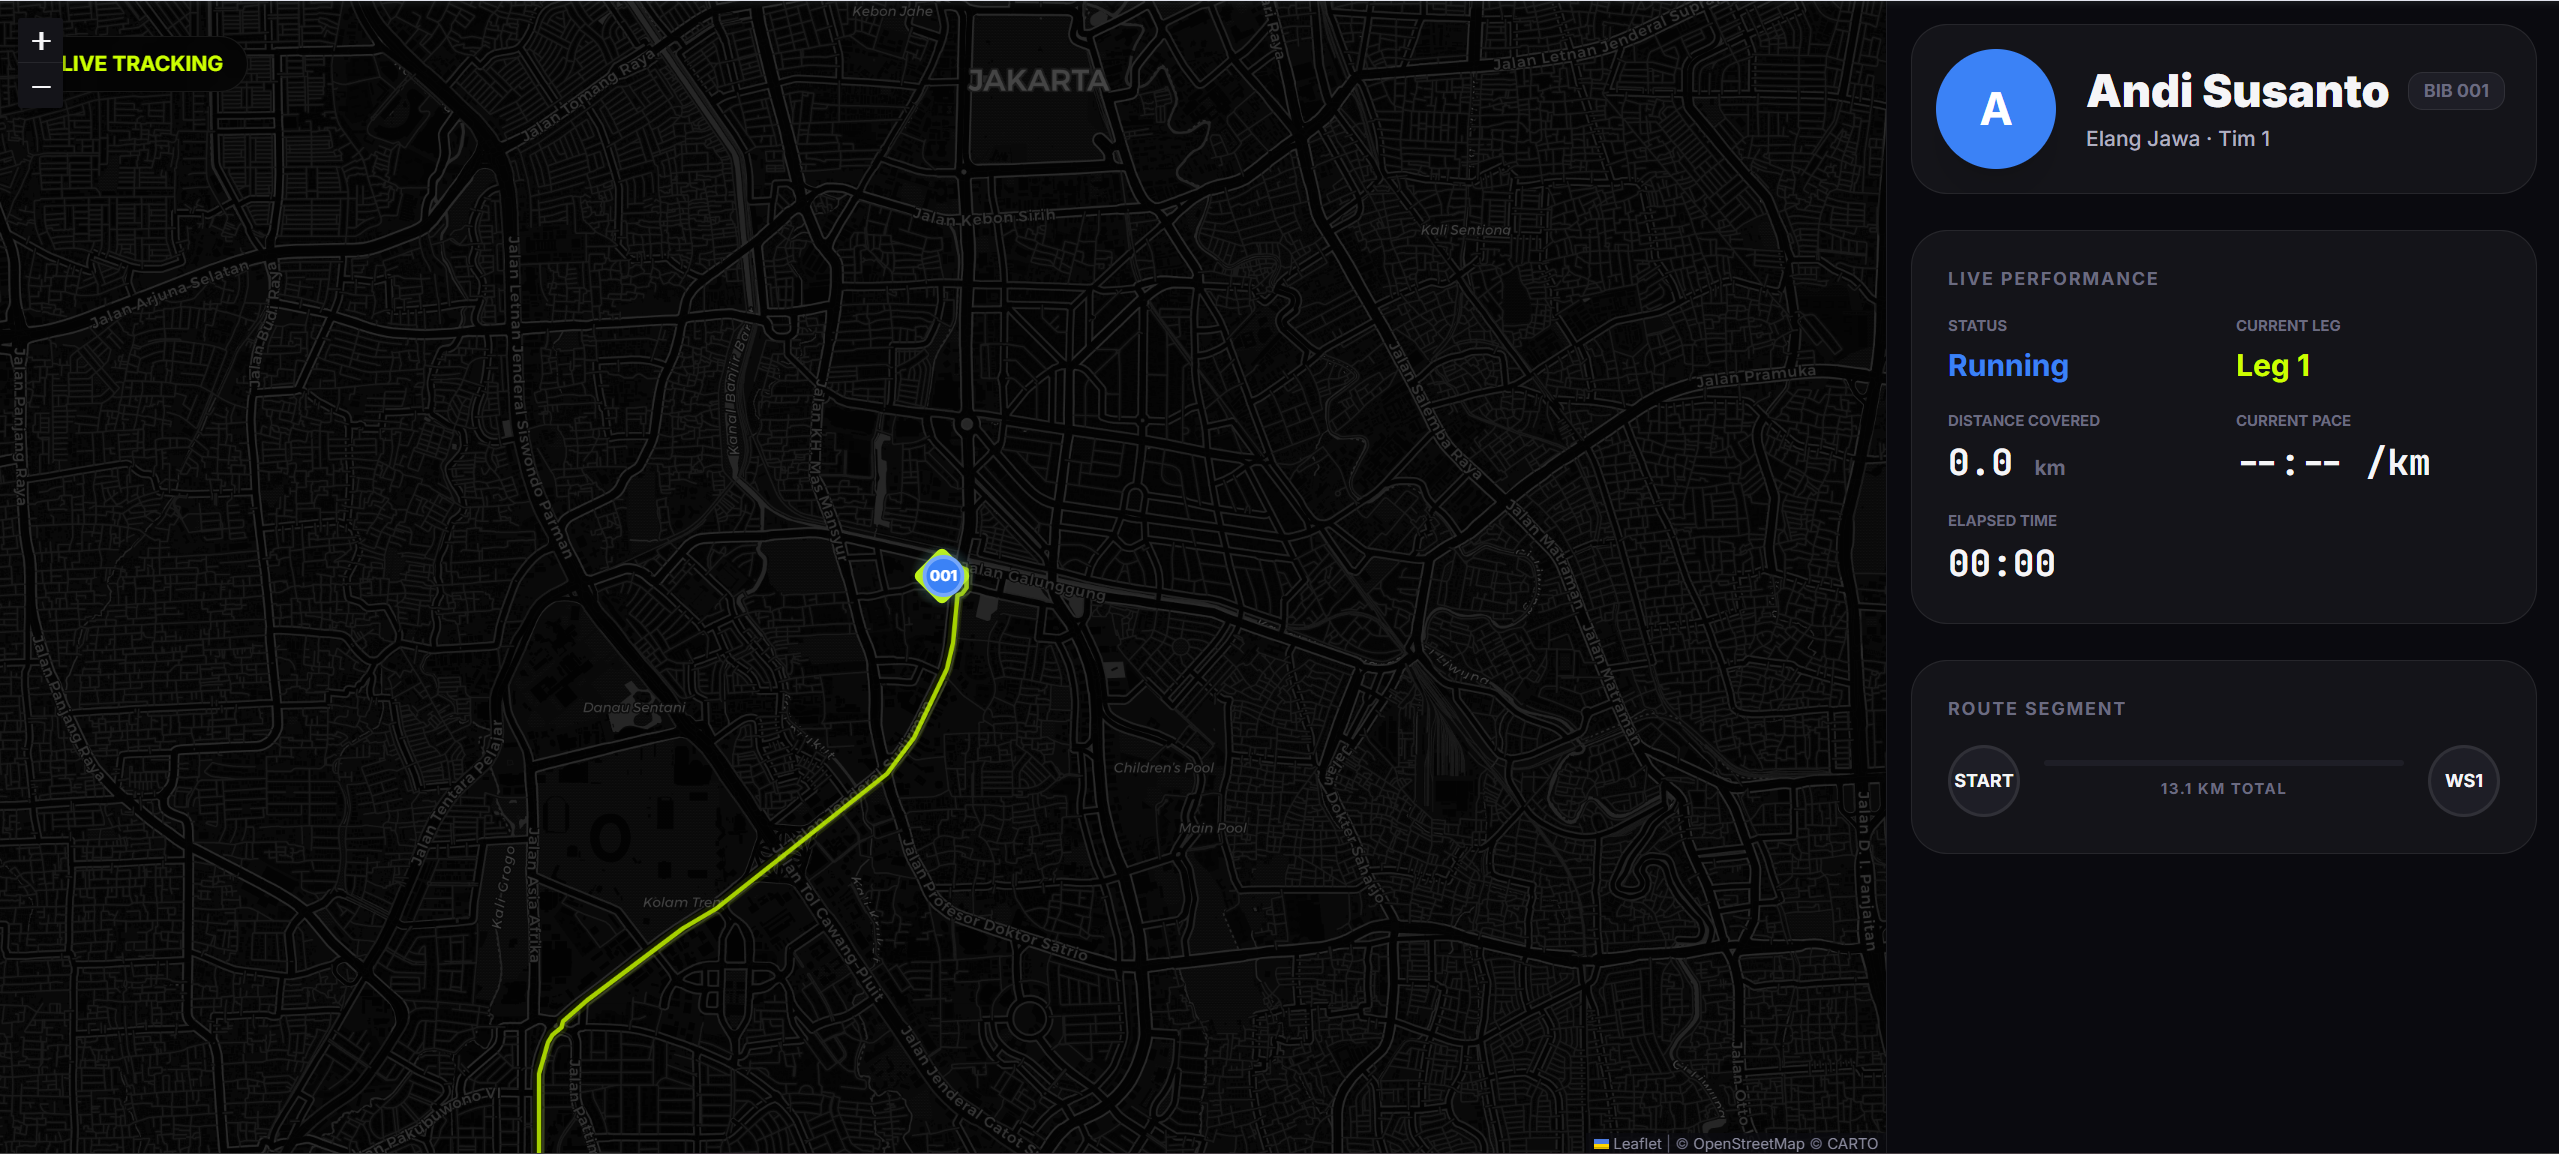
\includegraphics[width=0.62\textwidth,keepaspectratio]{images/implementasi/web/private-home.png} \\

\end{longtable}
